\documentclass[a4paper]{article} 
\addtolength{\hoffset}{-2.25cm}
\addtolength{\textwidth}{4.5cm}
\addtolength{\voffset}{-3.25cm}
\addtolength{\textheight}{5cm}
\setlength{\parskip}{0pt}
\setlength{\parindent}{0in}

\usepackage{blindtext} % Package to generate dummy text
\usepackage{charter} % Use the Charter font
\usepackage[utf8]{inputenc} % Use UTF-8 encoding
\usepackage{microtype} % Slightly tweak font spacing for aesthetics
\usepackage[english]{babel} % Language hyphenation and typographical rules
\usepackage{amsthm, amsmath, amssymb, amsfonts, nccmath} % Mathematical typesetting
\usepackage{float} % Improved interface for floating objects
\usepackage[final, colorlinks = true, 
linkcolor = black, 
citecolor = black]{hyperref} % For hyperlinks in the PDF
\usepackage{graphicx, multicol} % Enhanced support for graphics
\usepackage{xcolor} % Driver-independent color extensions
\usepackage{marvosym, wasysym} % More symbols
\usepackage{rotating} % Rotation tools
\usepackage{subcaption}
\usepackage{wrapfig}
% \usepackage{geometry}
\usepackage{censor} % Facilities for controlling restricted text
\newcommand{\note}[1]{\marginpar{\scriptsize \textcolor{red}{#1}}} % Enables comments in red on margin
\usepackage{bm}
\usepackage{blkarray}
\usepackage{enumitem}
\usepackage{pgfplots}
\usepackage{tikz}
\usetikzlibrary{bayesnet}

\usepackage{tcolorbox}
\usepackage[ruled,vlined]{algorithm2e}

\newcommand{\pd}[2]{\frac{\partial #1}{\partial #2}}
\newcommand{\loss}[0]{\mathcal{L}}
\newcommand{\chain}[3]{\frac{\partial #1}{\partial #2}\frac{\partial #2}{\partial #3}}
% \newcommand{\eq}[1]{\begin{equation*}\begin{split}#1\end{split}\end{equation*}}
\newcommand{\TODO}[1]{\textbf{\textcolor{red}{#1}}}
\newcommand{\E}[0]{\mathbb{E}} % Expectation
\newcommand{\R}[0]{\mathbb{R}} % Real numbers
\newcommand{\Cdo}[0]{\textnormal{do}}
\newcommand\independent{\protect\mathpalette{\protect\independenT}{\perp}}
\def\independenT#1#2{\mathrel{\rlap{$#1#2$}\mkern2mu{#1#2}}}
\newcommand*{\QED}{\hfill\ensuremath{\blacksquare}}%

\definecolor{green}{RGB}{0,160,0}
\definecolor{blue}{RGB}{0,0,160}
\definecolor{red}{RGB}{160,0,0}
\definecolor{orange}{RGB}{200,160,0}
\definecolor{purple}{RGB}{170,0,200}
\definecolor{cyan}{RGB}{0,200,200}
\definecolor{lightred}{RGB}{200,50,50}

\setcounter{tocdepth}{2}
% Title Page
\title{Summary Machine Learning 2}
\author{Phillip Lippe}


\begin{document}
\maketitle
\tableofcontents
\newpage

\section{Introduction to popular distributions and their properties}
\begin{itemize}
	\item This section (lecture 1 and 2) reviews different kinds of distributions, including the exponential family, Student-t distribution and common distributions for binary and discrete variables
	\item Furthermore, we shortly introduce Independent Component Analysis and Information theory
	\item In general, the first two lectures gave some fundamental knowledge we will use a couple of times for the rest of the course
	\item More mathematical tricks or examples of the exponential family can be found in the appendix
\end{itemize}
\subsection{Exponential family distributions}
\textbf{(Bishop 2.4)}
\begin{itemize}
	\item A distribution is considered a member of the exponential family if it can be written as follows:
	\begin{equation*}
	\tcbox[nobeforeafter]{\(
		\begin{split}
			p(\bm{x}|\bm{\eta}) & = h(\bm{x})g(\bm{\eta})\exp\left(\bm{\eta}^T \cdot \bm{u}(\bm{x})\right)\\[5pt]
			\bm{\eta} & \hspace{3mm}\text{natural parameters}\\
			\bm{u}(\bm{x}) & \hspace{3mm}\text{sufficient statistics}\\
		\end{split}
	\)}
	\end{equation*}
	\item $\bm{u}(\bm{x})$ is called sufficient statistics because for the maximum likelihood estimate of $\bm{\eta}$, it is sufficient to record $\sum_{n=1}^{N}\bm{u}(\bm{x}_n)$ instead of the whole dataset $\left\{\bm{x}_n\right\}_{n=1}^{N}$ (see below for ML estimate)
	\item An important property of the exponential families is that the moments of distributions (i.e. mean and variance) can be determined by deriving $-\ln g(\bm{\eta})$ by $\bm{\eta}$:
	\begin{equation*}
		\begin{split}
			\text{Normalization constant}\hspace{2mm} z(\bm{\eta}) & = \frac{1}{g(\bm{\eta})} = \int h(\bm{x})\exp\left(\bm{\eta}^T \cdot \bm{u}(\bm{x})\right) d\bm{x}\\
			\frac{\partial}{\partial \bm{\eta}} -\ln g(\bm{\eta}) & = -\frac{1}{z(\bm{\eta})} \int h(\bm{x})\bm{u}(\bm{x})\exp\left(\bm{\eta}^T \cdot \bm{u}(\bm{x})\right) d\bm{x} = \E[\bm{u}(\bm{x})\vert \bm{\eta}]\\
		\end{split}
	\end{equation*}
	\begin{itemize}
		\item Note that these moments are of the sufficient statistics $\bm{u}(\bm{x})$, and not $\bm{x}$
		\item Additionally, the second moment around the mean can be determined by: $\nabla_{\bm{\eta}}^2 -\ln g(\bm{\eta})$
	\end{itemize}
	\item From the first moment, we can show that the \underline{MLE solution} of the natural parameters are:
	$$\tcbox[nobeforeafter]{\(-\nabla_{\bm{\eta}}\ln g(\bm{\eta}) = \E[\bm{u}(\bm{x})\vert \bm{\eta}] \implies -\nabla_{\bm{\eta}}\ln g(\bm{\eta}_{\text{ML}}) = \frac{1}{N}\sum_{n=1}^{N} \bm{u}(\bm{x})\)}$$
\end{itemize}
\subsubsection{Conjugate priors}
\begin{itemize}
	\item A conjugate prior $p(\bm{\eta})$ is conjugate to the likelihood so that the posterior $p(\bm{\eta}|\bm{X})$ has the same form as the prior
	\item Each member of the exponential family has a conjugate prior
	\item To find the conjugate prior for a exponential distribution as likelihood, we only have to look at $\bm{\eta}$ of the likelihood and $\bm{u}(\bm{x})$ of the prior take on the same form. Then, we simply get:
	\begin{equation*}
		\begin{split}
			\bm{u}(\bm{x})_{\text{posterior}} & = \bm{\eta}_{\text{likelihood}} = \bm{u}(\bm{x})_{\text{prior}}\\
			\bm{\eta}_{\text{posterior}} & = \bm{u}(\bm{x})_{\text{likelihood}} + \bm{\eta}_{\text{prior}}
		\end{split}
	\end{equation*}
\end{itemize}
\subsubsection{Bayesian Inference for Gaussian}
\begin{itemize}
	\item We can demonstrate the conjugate prior idea for Gaussians (one dimensional), where we have to distinguish three cases
\end{itemize}
\begin{enumerate}
	\item \underline{Variance known, mean estimated}
	\begin{itemize}
		\item Conjugate prior is a Gaussian $p(\mu)=\mathcal{N}(\mu\vert\mu_0, \sigma_0^2)$ such that our posterior has the distribution:
		\begin{equation*}
		\tcbox[nobeforeafter]{\(
			\begin{split}
				& \textbf{Variance known, mean estimated}\\
				& p(\mu|\mathcal{D})=\mathcal{N}(\mu|\mu_N, \sigma_N^2), \hspace{5mm}\mu_N= \frac{\sigma^2 \mu_0 + N\sigma_0^2 \mu_{\text{ML}}}{N\sigma_0^2 + \sigma^2}, \hspace{5mm}\frac{1}{\sigma_N^2}=\frac{1}{\sigma_0^2} + \frac{N}{\sigma^2}
			\end{split}
		\)}
		\end{equation*}
	\end{itemize}
	\item \underline{Mean unknown, variance estimated}
	\begin{itemize}
		\item Conjugate prior for the precision $\lambda=\frac{1}{\sigma^2}$ is a Gamma distribution $\text{Gamma}(\lambda|a_0, b_0)$ such that the posterior is:
		\begin{equation*}
		\tcbox[nobeforeafter]{\(
			\begin{split}
			& \textbf{Mean known, variance estimated}\\
			& p(\lambda|\mathcal{D})=\text{Gamma}(\lambda|a_N,b_N), \hspace{5mm}a_N=a_0+\frac{N}{2},\hspace{5mm}b_N = b_0+\frac{1}{2}\sum_n(x_n-\mu)^2
			\end{split}
			\)}
		\end{equation*}
	\end{itemize}
	\item \underline{Variance and mean estimated}
	\begin{itemize}
		\item If both are unknown, we have a ``normal-Gamma'' distribution as prior and posterior: $p(\mu,\lambda|a,b,\mu_0, \beta)=\mathcal{N}(\mu|\mu_0, (\beta \lambda^{-1}))\text{Gamma}(\lambda|a,b)$
		\item Finding the posterior is harder in this case because of the combined distribution. For details, see Bishop, but in the lecture it was not further discussed
	\end{itemize}
\end{enumerate}
\subsection{Student's-t distribution}
\begin{itemize}
	\item The Student-t distribution is "heavy-tailed", meaning that the probability for data points decreases slower with the distance from the mean/center than for a Gaussian (polynomial $\text{St}(x)\propto |x|^{-\alpha}$ instead of exponential $\mathcal{N}\propto e^{-\frac{x^2}{\sigma^2}}$)
	\item This makes the distribution more \underline{robust against outliers} as the MLE solution is less influenced by those and focuses more on the biggest data point mass (see Figure~\ref{fig:exponential_families_student_t})
	\begin{figure}[ht!]
		\centering
		\begin{subfigure}{0.25\textwidth}
			\centering
			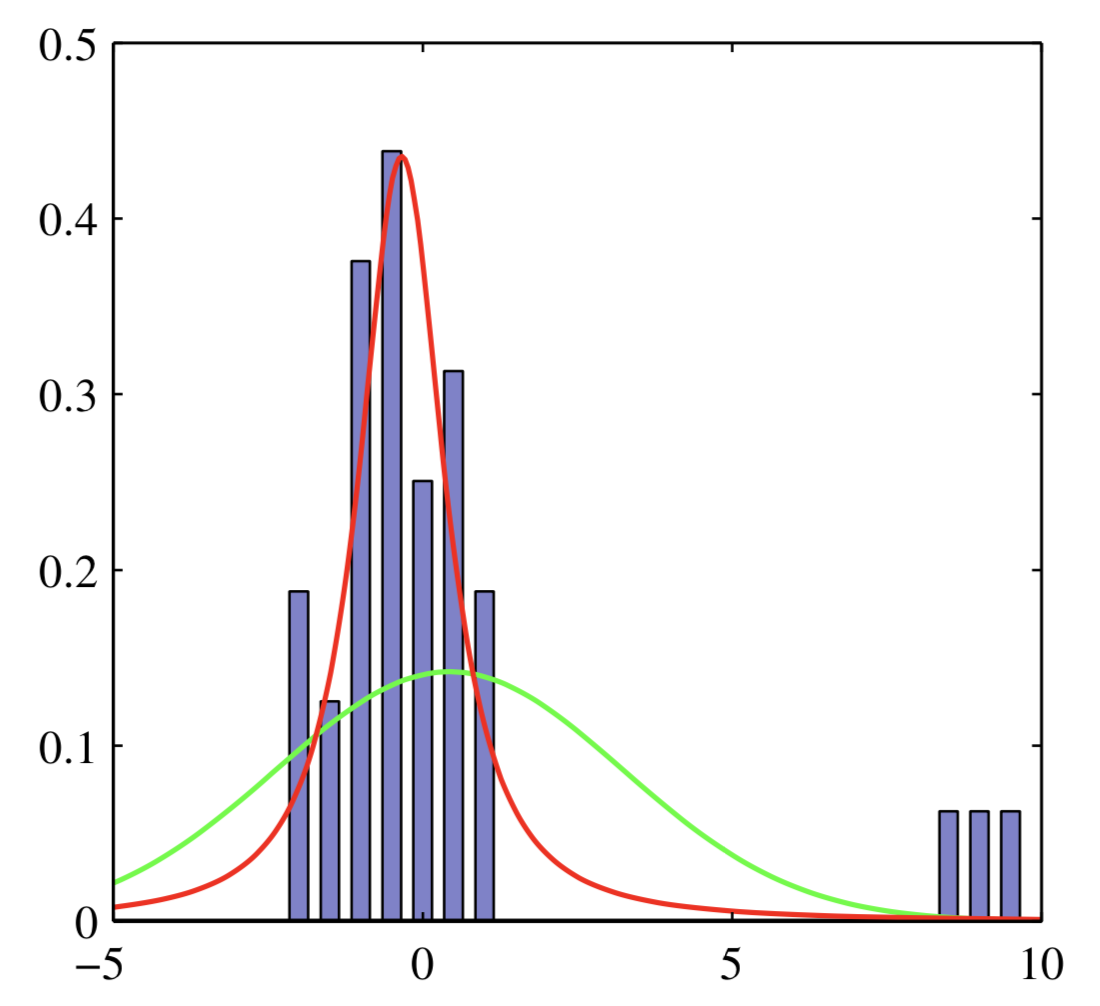
\includegraphics[width=\textwidth]{figures/exponential_families_student_t.png}
			\caption{MLE estimate}
			\label{fig:exponential_families_student_t}
		\end{subfigure}
		\hspace{10mm}
		\begin{subfigure}{0.3\textwidth}
			\centering
			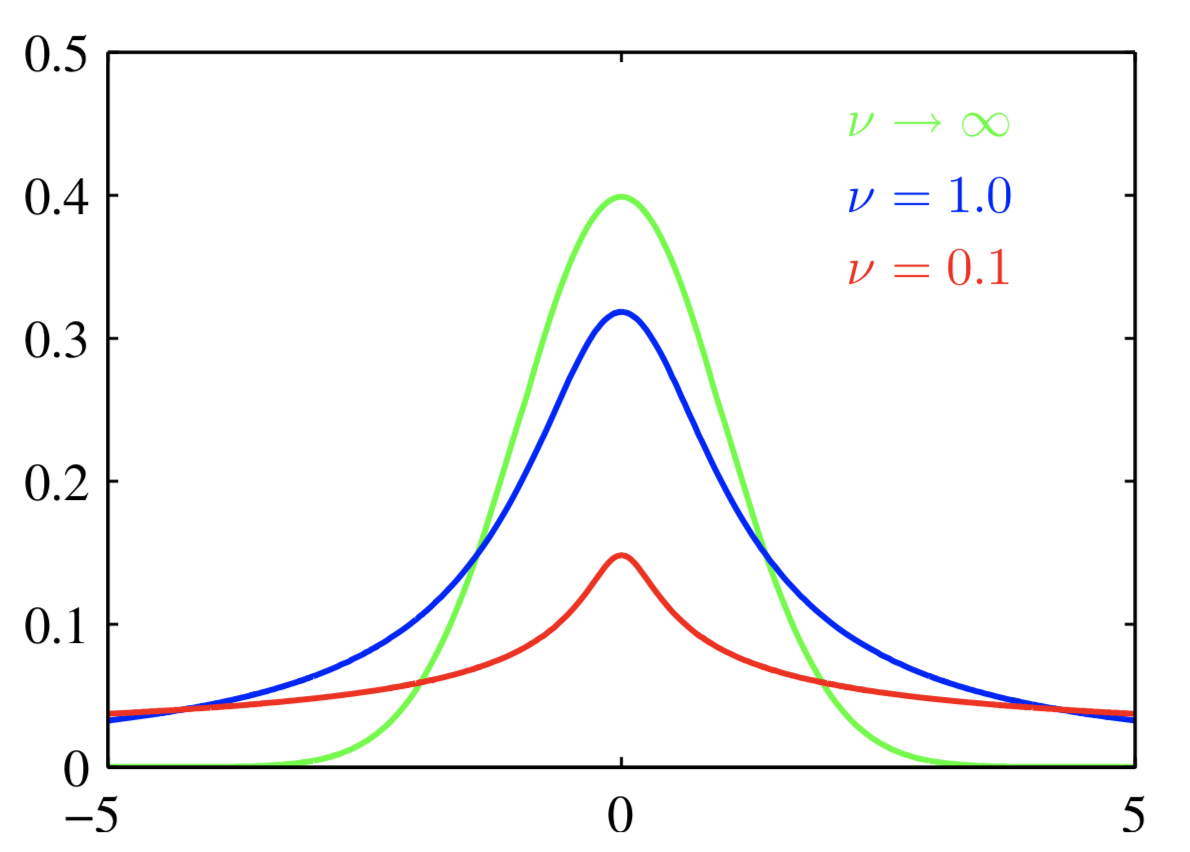
\includegraphics[width=\textwidth]{figures/exponential_families_student_t_nu.png}
			\caption{Effect of parameter $\nu$}
			\label{fig:exponential_families_student_t_nu}
		\end{subfigure}
		\caption{(a) Comparison of MLE solution of Student-t distribution (red) and Gaussian (green). (b) The parameter $\nu$ for fixed $\mu=0$ and $\lambda=1$. For $\nu\to\infty$, }
	\end{figure}
	\item It emerges from a infinite mixture of Gaussians with a fixed mean and the precision (i.e. inverse variance) distributed as a Gamma distribution:
	\begin{enumerate}
		\item Draw precision $\tau \sim \text{Gamma}(a,b)$
		\item Draw $x\sim \mathcal{N}(\mu, \tau^{-1})$
	\end{enumerate}
	Then the resulting $x$ will be distributed according to the Student-t distribution
	$$p(x) \sim \text{St}(x\mid \mu, \lambda=a/b, \nu=2a)$$
	\item By marginalizing out $\tau$, we can derivate the PDF of the student distribution:
	\begin{equation*}
		\begin{split}
			\text{Scalar}\hspace{2mm}&\text{St}(x\mid\mu, \lambda=a/b, \nu=2a) = \frac{b^a}{\Gamma(a)\sqrt{2\pi}}\left(b + \frac{(x-\mu)^2}{2}\right)^{-a-\frac{1}{2}}\Gamma\left(a+\frac{1}{2}\right)\\[8pt]
			\text{d-dimensional}\hspace{2mm} &  \text{St}(\bm{x}\mid\bm{\mu}, \bm{\Sigma}, \nu) = \frac{\Gamma\left(\frac{d}{2} + \frac{\nu}{2}\right)}{\Gamma\left(\frac{d}{2}\right)}\frac{1}{\left(\pi\nu\right)^{d/2}\left|\bm{\Sigma}\right|^{1/2}}\left(1+\nu^{-1}\left(\bm{x}-\bm{\mu}\right)^T \bm{\Sigma}^{-1}\left(\bm{x}-\bm{\mu}\right)\right)^{-\frac{d}{2}-\frac{\nu}{2}}\\
		\end{split}
	\end{equation*}
	\item The parameter $\lambda$ is often called precision, but does not exactly represent the inverse of the variance.
	\item $\nu$ is called the degrees of freedom (see Figure~\ref{fig:exponential_families_student_t_nu}). For $\nu\to\infty$, the student-t distribution becomes a Gaussian $\mathcal{N}(x\vert\mu, \lambda^{-1})$
\end{itemize}
\subsection{Distributions for Binary and Discrete Variables}
\begin{itemize}
	\item In this section, we review common distributions for binary and discrete distributions. We can actually find one-to-one correlations in the binary and categorical space:
	\begin{table}[ht!]
		\centering
		\begin{tabular}{c|c}
			Binary & Discrete\\\hline
			Bernoulli & Categorical\\
			Binomial & Multinomial\\
			Beta & Dirichlet
		\end{tabular}
		\vspace{-5mm}
	\end{table}
\end{itemize}
\subsubsection{Binary}
\begin{description}
	\item[Bernoulli distribution] can be interpreted as a coin flip, and models a single binary outcome:
	$$\text{Bern}(x|\mu)=\mu^{x}(1-\mu)^{1-x}, \hspace{3mm}x\in\{0,1\}$$
	\begin{itemize}
		\item Expectation $\E[x|\mu]=\mu$
		\item Variance $\mathbb{V}\text{ar}[x]=\E[x^2]-\E[x]^2=\mu(1-\mu)$
		\item Maximum likelihood estimate $\mu_{\text{ML}}=\frac{1}{N}\sum_{n=1}^{N} x_n$ (sensitive to overfitting for small dataset)
		\item Exponential family $p(x|\eta)=\sigma(-\eta)\exp(\eta\cdot x), \eta=\ln \frac{\mu}{1-\mu}$
	\end{itemize}

	\item[Binomial distribution] models $N$ i.i.d. Bernoulli experiments, where we define $m$ as $m=\sum_{i=1}^{N}x_i$, i.e. the number of times the outcome is $1$:
	$$\text{Bin}(m|N,\mu)=\frac{N!}{(N-m)!m!}\mu^{m}(1 - \mu)^{N-m}$$	
	\begin{itemize}
		\item Expectation $\E[m]=\sum_{i=1}^{N}\E[x_i]=N\cdot \mu$
		\item Variance $\mathbb{V}\text{ar}[x]=N\cdot \mu(1-\mu)$
		\item Maximum likelihood estimate $\mu_{\text{ML}}=\frac{m}{N}$
		\item Exponential family $p(m|\eta)=\frac{N!}{(N-m)!m!}\cdot \exp(N\log \log 1-\mu) \cdot \exp(m\log\frac{\mu}{1-\mu})$, $\eta=\log \frac{\mu}{1-\mu}$
		\item Conjugate prior: Beta distribution. The posterior is: $\text{Beta}(\mu|a+m,b+N-m)$
	\end{itemize}

	\item[Beta distribution] is the conjugate prior for the binomial distribution
	$$\text{Beta}(\mu|a,b)=\frac{\Gamma(a+b)}{\Gamma(a)\Gamma(b)}\mu^{a-1}(1-\mu)^{b-1}$$
	\begin{itemize}
		\item Expectation $\E[\mu]=\frac{a}{a+b}$
		\item Variance $\mathbb{V}\text{ar}[x]=\frac{ab}{(a+b)^2(a+b+1)}$
		\item Exponential family: see Appendix
	\end{itemize}
\end{description}
\subsubsection{Discrete}
\begin{description}
	\item[Categorical distribution] considers a single sample, and assign each category a different probability. The input $\bm{x}$ is a one-hot vector.
	$$\text{Cat}(\bm{x}|\bm{\mu})=\prod_{k=1}^{K}\mu_k^{x_k}=\mu_{x_k}, \hspace{3mm}\sum_k \mu_k = 1$$
	 \begin{itemize}
	 	\item Expectation $\E[\bm{x}]=\bm{\mu}$
	 	\item Covariance $\text{Cov}[\bm{x}]=\text{diag}(\bm{\mu}(1-\bm{\mu}))$
	 	\item Maximum likelihood estimate  $\bm{\mu}_{\text{ML}}=\frac{1}{N}\sum_{i=1}^{N} \bm{x}$
	 	\item Exponential family $p(\bm{x}|\bm{\eta})=\frac{1}{1+\sum_{k=1}^{K-1}\exp(\eta_k)}\cdot \exp(\bm{\eta}^T\bm{x})$, $\eta_k=\ln\frac{\mu_k}{1-\sum_{j=1}^{K-1}\mu_j}$
	 \end{itemize}
	\item[Multinomial distribution] takes $N$ i.i.d. categorical observations into account, where $m_k=\sum_{n=1}^{N} x_{nk}$.
	$$\text{Mult}(m_1,...,m_K|N,\bm{\mu})=\frac{N!}{\prod_{k=1}^{K}m_k!}\prod_{k=1}^{K} \mu_{k}^{m_k}$$
	\begin{itemize}
		\item Expectation: $\E[\bm{x}]=N\cdot \mu$
		\item Covariance: $\text{Cov}[\bm{x},\bm{x}]=N(\text{diag}(\bm{\mu})-\bm{\mu}\bm{\mu}^T)$
		\item Maximum likelihood estimation: $\bm{\mu}_{\text{ML}}=\frac{\bm{m}}{N}$
		\item Exponential family: see Appendix
	\end{itemize}
	\item[Dirichlet distribution] is the conjugate prior for multinomial
	$$\text{Dir}(\bm{\mu}|\bm{\alpha})=\frac{\Gamma(\sum_k \alpha_k)}{\prod_k
	\Gamma(\alpha_k)} \prod_{k=1}^{K}\mu_k^{\alpha_k-1}$$
	\begin{itemize}
		\item Expectation $\E[\bm{x}]=\frac{1}{\sum_k \alpha_k}\bm{\alpha}$
		\item Covariance $\text{Cov}[\bm{x}]=-\frac{1}{\sum_k \alpha_k + 1}\bm{\alpha}\bm{\alpha}^T$
		\item Exponential family: see Appendix
	\end{itemize}
\end{description}
\subsection{Independent Component Analysis}
\begin{itemize}
	\item Independent Component Analysis (ICA) tries to reconstruct source signals from linearly mixed measurements. For example, for two sources $S(t)=\begin{bmatrix}
	S_1(t)\\S_2(t)
	\end{bmatrix}$, we assume to have the measurements:
	$$X(t)=\begin{bmatrix}
	X_1(t)\\X_2(t)
	\end{bmatrix} = \begin{bmatrix}
	\alpha_1 S_1(t) + \beta_1 S_2(t)\\\alpha_2 S_2(t) + \beta_2 S_2(t)
	\end{bmatrix}$$
	The goal is now to find the parameter matrix
	$$\bm{A}=\begin{bmatrix}
	\alpha_1 & \beta_1\\ \alpha_2 & \beta_2
	\end{bmatrix}$$
	to reconstruct our signals $S(t)$ from the measurements $\bm{X}(t)=\bm{A}\bm{S}(t)$
	\item Note that we can only reconstruct $S(t)$ up to permutation and scaling/multiplicative factors as these give the same result
	\item As we assume the sources to be independent, we can write the joint probability distribution as:
	$$p(S_1,...,S_I)=\prod_{i=1}^{I}p(S_i)$$
	One crucial element of ICA is that these prior distributions need to be designed by the user. This requires pre-knowledge of how the source signals can look like (e.g. Gaussian, bounded Uniform, etc.). The performance of the algorithm depend on this design choice, and can lead to ICA failing if the prior has a very different distribution than points in the sources.
	\item We will again use a maximum likelihood  approach where we try to increase the probability of the observed data, which can be derived as:
	$$\ln p(\bm{x}|\bm{A})=\ln |\det \bm{A}| + \frac{1}{N}\sum_{n=1}^{N}\sum_{i=1}^{I}\ln p_i\left(\sum_{j=1}^{I} \left(A^{-1}\right)_{ij} x^{(n)}_j\right)$$
	For simplicity, we replace $\bm{A}^{-1}=\bm{W}$, and aim to learn $\bm{W}$ which is slightly easier.
	\item We take now the derivative with respect to $\bm{W}$, and end up with the following expression:
	$$\bm{W}^{t+1}=\bm{W}^{t} + \alpha \cdot \frac{1}{N}\sum_{n=1}^{N}\left(\nabla_{\bm{S}} \log p(\bm{S})\Big\vert_{S=S_n}\bm{S}_n^T+\bm{I}\right)\bm{W}$$
	where we estimate $\bm{S}=\bm{W}\bm{X}$. In addition, we see here that what we actually need from our prior is the derivative of its log. Hence, the prior is mostly designed to have a simple form of $\Phi_i=\frac{\partial \ln p_i(a_i)}{\partial a_i}$.
	\item We can slightly simplify the gradient calculation by splitting it into multiple parts. Summarizing the full algorithm, we get:
	\begin{tcolorbox}[colback=white!80!gray,colframe=gray!75!black,title=Independent Component Analysis]
		\begin{algorithm}[H]
			\SetAlgoLined
			Choose prior and calculate log derivative $\Phi_i=\frac{\partial \ln p_i(a_i)}{\partial a_i}$\;
			Set learning rate $\eta$\;
			Initialize $\bm{W}=\bm{A}^{-1}$\;
			\While{$\nabla \bm{W}^{(t)} > \epsilon$}{
				Let $\hat{\bm{S}}=\bm{W}\bm{X}$ be the current estimate of $\bm{S}$\;
				Let $\bm{Z}_i=\Phi_i(\hat{\bm{S}}_i)$\;
				Let $\bm{X}' = \bm{W}^T\hat{\bm{S}}$\;
				Calculate the gradients $\nabla \bm{W}^{(t)}= \bm{W}^{(t)} + \frac{1}{N}\left[ \bm{Z}{\bm{X}'}^T\right]$\;
				Apply gradient with learning rate $\bm{W}^{(t+1)}=\bm{W}^{(t)}+\eta \nabla \bm{W}^{(t)}$\;
			}
			Reconstruct signals $\bm{S}_n=\bm{W}\bm{X}_n$\;
		\end{algorithm}
	\end{tcolorbox} 
	\item One issue with ICA is that the signals are not allowed to be Gaussian. If this would be the case, we can not reconstruct the signal up to rotation as Gaussians are rotation invariant. Hence, the signals will be messed up although we find an optimum
\end{itemize}
\subsection{Information theory}
\begin{itemize}
	\item The information of an event $A$ can be measured by:
	\begin{equation*}
		\begin{split}
			h(A) & = -\log_2 p(A)\hspace{4mm}\text{(in bits)}\\
			& = - \ln p(A)\hspace{4mm}\text{(in nats)}
		\end{split}
	\end{equation*}
	\item An important measurement of a distribution in information theory is the Shannon entropy, which can be interpreted as the expected information of an event according to the distribution $p$:
	\begin{equation*}
		\tcbox[nobeforeafter]{\(
			H(X) = -\sum_{x\in D_x} p(x)\log_2 p(x)
		\)}
	\end{equation*}
	In case we have $N$ independent events, the entropy is the sum of the single entropy of each of the $N$ events.
	\item The entropy can also be defined for continuous space. It is then referred to as the differential entropy:
	$$H(\bm{x})=-\int p(\bm{x})\log_2 p(\bm{x})d\bm{x}$$
	\item We can also define conditional entropy, which is as follows:
	\begin{equation*}
	\tcbox[nobeforeafter]{\(
		H(\bm{x}|\bm{y}) = -\int p(\bm{x})\left[\int p(\bm{y}|\bm{x})\ln p(\bm{y}|\bm{x})d\bm{y}\right]d\bm{x}
		\)}
	\end{equation*}
	with the property $H(\bm{x},\bm{y})=H(\bm{x})+H(\bm{y}|\bm{x})=H(\bm{y})+H(\bm{x}|\bm{y})$
	\item Another well-known measurement is the Kullback-Leiber divergence (also referred to as relative entropy):
	\begin{equation*}
		\tcbox[nobeforeafter]{\(
			\text{KL}(p(\bm{x})||q(\bm{x})) = -\int p(\bm{x})\ln \frac{q(\bm{x})}{p(\bm{x})}d\bm{x}
		\)}
	\end{equation*}
	Some properties of this divergence are:
	\begin{itemize}
		\item Always positive: $\text{KL}(p||q)\geq 0$
		\item If $\text{KL}(p||q) = 0$, then $p=q$ (if $p$,$q$ are sufficient regular, i.e. strictly positive and integral defined)
		\item The triangular inequality does not hold for KL, thus it is not a distance measure: 
		
		$\text{KL}(p||q)+\text{KL}(q||r)\not\geq \text{KL}(p||r)$
	\end{itemize}
	\item Mutual information describes the amount of information that is shared among $x$ and $y$:
	\begin{equation*}
		\tcbox[nobeforeafter]{\(
			I(\bm{x};\bm{y}) = \text{KL}(p(\bm{x},\bm{y})||p(\bm{x}),p(\bm{y})) = H(\bm{x})-H(\bm{x}|\bm{y}) = H(\bm{y}) - H(\bm{y}|\bm{x})
		\)}
	\end{equation*}
	In other words, how much information about $y$ do I get by observing $x$. In a diagram, mutual information can be visualized as follows:
	\begin{figure}[ht!]
		\centering
		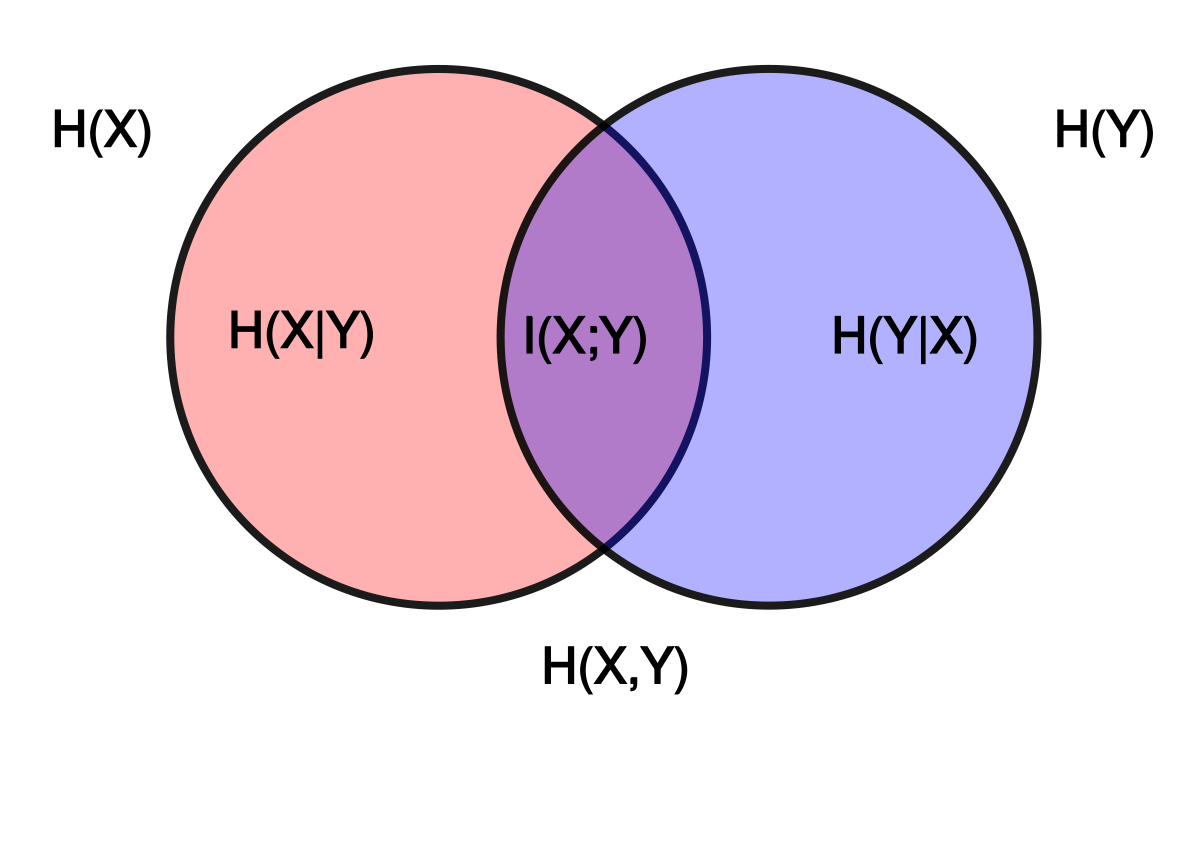
\includegraphics[width=0.3\textwidth]{figures/information_theory_mutual_information.png}
		\caption{Visualizing the relationship between mutual information and entropy.}
	\end{figure}
\end{itemize}

\newpage
\section{Probabilistic graphical models}
\begin{itemize}
	\item It is often beneficial to visualize a probabilistic model as a diagram, which we call \textit{(probabilistic) graphical models}. 
	\item They are good for:
	\begin{itemize}
		\item causal reasoning/modeling
		\item calculating inference and conditional distributions efficiently 
		\item Designing and communicating statistical model
		\item Encoding (conditional) independence relations
	\end{itemize} 
	\item Note that there are often multiple ways to express the same probability distribution. For example, take a joint distribution $p(A,B,C)$, which we can either write as $p(A,B,C)=p(A)p(B|A)p(C|A,B)$ (see Figure~\ref{fig:graphical_models_example_1}) or $p(A,B,C)=p(C)p(A|C)p(B|A,C)$ (see Figure~\ref{fig:graphical_models_example_2}). Nevertheless, what we are interested in is the graphical representation with the least number of edges, as e.g. if $A$ and $B$ are independent (conditionally on $C$), we can drop the edge between those.
	\begin{figure}[ht!]
		\centering
		\begin{subfigure}{0.4\textwidth}
			\centering
			\tikz{ %
				\node[latent] (A) {$A$} ; %
				\node[latent, right=of A] (B) {$B$} ; %
				\node[latent, below=of B] (C) {$C$} ; %
				
				\edge{A}{B};
				\edge{A}{C};
				\edge{B}{C};
			}
			\caption{$p(A,B,C)=p(A)p(B|A)p(C|A,B)$}
			\label{fig:graphical_models_example_1}
		\end{subfigure}
		\hspace{10mm}
		\begin{subfigure}{0.4\textwidth}
			\centering
			\tikz{ %
				\node[latent] (A) {$A$} ; %
				\node[latent, right=of A] (B) {$B$} ; %
				\node[latent, below=of B] (C) {$C$} ; %
				
				\edge{A}{B};
				\edge{C}{A};
				\edge{C}{B};
			}
			\caption{$p(A,B,C)=p(C)p(A|C)p(B|A,C)$}
			\label{fig:graphical_models_example_2}
		\end{subfigure}
		\caption{Two different graphical models (here Bayesian Networks) for the same joint distribution $p(A,B,C)$.}
	\end{figure}
	\item We distinguish between directed acyclic graphs, which we call \textit{Bayesian networks} (BN), and undirected graphs, which are \textit{Markov Random Fields} (MRF)
\end{itemize}

\subsection{Bayesian Networks}
\begin{itemize}
	\item There is a simple way for creating a Bayesian network for a given statistical model.
	\begin{enumerate}
		\item Determine the ordering of the variables (``\textit{topological ordering}'')
		\item In this ordering, call the parents of the random variable $X_i$: $\text{pa}_i$, or $\text{pa}(X_i)$ which is a subset of variables with lower ordering: $\text{pa}_i \subseteq \left\{1,...,i-1\right\}$. The joint probability distribution can be written as:
		$$p(X_1,...,X_M) = \prod_{i=1}^{M}p(X_i|X_{\text{pa}_i})$$
		\item In the graphical model, draw an edge from $X_j$ to $X_i$ if $j\in \text{pa}_i$
	\end{enumerate}
	\item \underline{Example}: (first-order) Markov Chain
	\begin{itemize}
		\item The joint probability distribution of a Markov Chain can be expressed by:
		$$p(X_1,...,X_M)=p(X_1)\cdot \prod_{i=2}^{M} p(X_i|X_{i-1})$$
		\item The corresponding Bayesian Network looks as follows:
		\begin{figure}[ht!]
			\centering
			\tikz{ %
				\node[obs] (x1) {$X_1$} ; %
				\node[obs, right=of x1] (x2) {$X_2$} ; %
				\node[obs, right=of x2] (x3) {$X_3$} ; %
				\node[const, right=of x3] (xetc1) { \hspace{2mm}...\hspace{2mm} } ; %
				\node[obs, right=of xetc1] (xM) {$X_M$} ; %
				
				\edge{x1}{x2};
				\edge{x2}{x3};
				\edge{x3}{xetc1};
				\edge{xetc1}{xM};
			}
		\end{figure}
	
		where the filling expresses that $X_i$ is an observed variable.
	\end{itemize}
	\item \underline{Example}: Regression
	\begin{itemize}
		\item Suppose we have a simple regression problem where we want to learn parameters $W$ to predict targets $T$ from input $X$. We further assume that we know our sensory noise $\sigma^2$, and have a prior with hyperparameters $\alpha$.
		\item 
		\begin{figure}[ht!]
			\centering
			\tikz{ %
				\node[obs] (x) {$X_n$} ; %
				\node[obs, right=of x] (t) {$T_n$} ; %
				\plate{xt}{(x)(t)}{$n=1,...,N$};
				
				\node[latent, above=of t] (w) {$W$} ; %
				\node[const, left=of w] (alpha) {$\alpha$} ; %
				\node[const, right=of t] (sigma) {$\sigma^2$} ; %
				
				\edge{x}{t};
				\edge{w}{t};
				\edge{alpha}{w};
				\edge{sigma}{t};
			}
		\end{figure}
	
		We can express this in the graphical model above, which represents the probability distribution
		$$p(W, \left\{T_n\right\}, \left\{X_n\right\}|\alpha, \sigma^2)p(W|\alpha)\prod_{n=1}^{N} \left[p(T_n|X_n, W, \sigma^2)p(X_n)\right]$$
		Note that in the graphical model, $\alpha$ and $\sigma^2$ are assumed to be fixed and known, and the ``plate'' can be interpreted as copying the content $N$ times (i.e. we have $N$ $X_i$ and $T_i$ variables with the same edges).
		
		Also, if desired, we could have used a constant for the data points $X_i$ as well as these are often assumed to be fixed.
		\item If we also want to express the predictive distribution $p(T^{*}|X^{*},W, \left\{T_n\right\}, \left\{X_n\right\},\alpha, \sigma^2)$, we can extend our model as follows:
		\begin{figure}[ht!]
			\centering
			\tikz{ %
				\node[obs] (x) {$X_n$} ; %
				\node[obs, right=of x] (t) {$T_n$} ; %
				\plate{xt}{(x)(t)}{$n=1,...,N$};
				
				\node[latent, above=of t] (w) {$W$} ; %
				\node[const, left=of w] (alpha) {$\alpha$} ; %
				\node[const, right=of t] (sigma) {$\sigma^2$} ; %
				
				\node[latent, right=of w] (tstar) {$T^{*}$} ; %
				\node[obs, right=of tstar] (xstar) {$X^{*}$} ; %
				
				
				\edge{x}{t};
				\edge{w}{t};
				\edge{w}{tstar};
				\edge{xstar}{tstar};
				\edge{alpha}{w};
				\edge{sigma}{t};
				\edge{sigma}{tstar};
			}
		\end{figure}
	\end{itemize}
\end{itemize}
\subsubsection{Conditional independence and D-separation}
\begin{itemize}
	\item A useful property of graphical models is that we can easily study the independence relations between random variables in our model. 
	\item We call $X$ and $Y$ being independent iff $p(X,Y)=p(X)p(Y)$. The notation for this is $X\independent Y$
	\item $X$ is \textit{conditionally} independent of $Y$ given $Z$ if $p(X,Y|Z)=p(X|Z)p(Y|Z)$. The notation for this is $X\independent Y|Z$. Note that if $X$ and $Y$ are generally independent, we can also write $X\independent Y|\emptyset$
	\item For proving/testing conditional independence, we can use \textbf{d-separation}. Supposed $A$, $B$, $C$ are sets of variables. If $A$ is d-separated from $B$ given $C$, then $p(X_A,X_B|X_C)=p(X_A|X_C)p(X_B|X_C)$, which we can also write as $A\perp B|C\implies X_A\independent X_B|X_C$ 
	\item Note that the other way round, $X_A\independent X_B|X_C\not\Rightarrow A\perp B|C $ is not always valid (but mostly) as we will show in a later example. Hence, if $A$ and $B$ are not d-separated, it does not necessarily mean that $X_A$ and $X_B$ are not conditional independent.
	
	\item The algorithm can be summarized as follows:
	\begin{tcolorbox}[colback=white!85!gray,colframe=gray!75!black,title=D-separation]
		Given the sets of variables $A$, $B$, $C$:
		\begin{enumerate}
			\item Consider all paths (sequence of nodes, connected by edges,  s.t. no node repeats) between any node in $A$ and any node in $B$
			\item Mark a path as \underline{blocked} by $C$ if
			\begin{enumerate}
				\item It contains a collider $...\rightarrow u \leftarrow ...$ such that $u$ is not an ancestor of a node in $C$
				\item It contains a non-collider $...\rightarrow u$, $...\rightarrow u \rightarrow ...$, $...\leftarrow u \rightarrow ...$ such that $u$ is in $C$
			\end{enumerate}
			\item If all paths are marked as blocked by $C$, then $A$ is d-separated from $B$ given $C$
		\end{enumerate}
	\end{tcolorbox}	
	\item \underline{Examples}: 
	\begin{itemize}
		\item Consider the following graphical model:
		\begin{figure}[ht!]
			\centering
			\tikz{ %
				\node[latent] (xA) {$X_A$} ; %
				\node[latent, right=of xA] (xB) {$X_B$} ; %
				\node[latent, below=of xB] (xC) {$X_C$} ; %
				
				\edge{xC}{xA};
				\edge{xC}{xB};
			}
		\end{figure}
	
		$A$ is d-separated from $B$ given $C$ as the only way from $B$ to $A$ is through $X_C$, and it represents a non-collider: $X_A\independent X_B|X_C$.
		
		Note that $A$ is not d-separated from $B$ given $\emptyset$ because $X_C$ is then neither a non-collider nor a collider.
		\item Consider the following graphical model:
		\begin{figure}[ht!]
			\centering
			\tikz{ %
				\node[latent] (xA) {$X_A$} ; %
				\node[latent, right=of xA] (xC) {$X_C$} ; %
				\node[latent, right=of xC] (xB) {$X_B$} ; %
				
				\edge{xA}{xC};
				\edge{xC}{xB};
			}
		\end{figure}
	
		Similarly to the previous model, $A$ is d-separated from $B$ given $C$ as the only way from $B$ to $A$ is through $X_C$, and it represents a non-collider: $X_A\independent X_B|X_C$.
		
		However, here we can show a special case where conditional independence does not imply d-separation. Suppose that we model $p(C|A)=\delta_{C,A}$, hence being a deterministic mapping. Now, $C\independent B|A$ holds because if we know $A$, we know $C$ for certain. Nevertheless, the d-separation is not valid because there is a direct path from $C$ to $B$! 
		
		\item Consider the following graphical model:
		\begin{figure}[ht!]
			\centering
			\tikz{ %
				\node[latent] (xA) {$X_A$} ; %
				\node[latent, right=of xA] (xC) {$X_C$} ; %
				\node[latent, above=of xC] (xB) {$X_B$} ; %
				\node[const, right=of xC] (xetc) {\hspace{2mm}...\hspace{2mm} } ; %
				\node[latent, right=of xetc] (xD) {$X_D$} ; %
				
				\edge{xA}{xC};
				\edge{xB}{xC};
				\edge{xC}{xetc};
				\edge{xetc}{xD};
			}
		\end{figure}
	
		$A$ is d-separated from $B$ given the empty set as $X_C$ represents a collider which is not in the empty set: $X_A\independent X_B|\emptyset$.
		
		$A$ is \textit{not} d-separated from $B$ given $C$ because $X_C$ is then not a collider anymore: $A\not\perp B|C$.
		
		$A$ is \textit{not} d-separated from $B$ given $D$ because $X_C$ is an ancestor of a node in $D$, and hence, not a collider: $A\not\perp B|D$.
	\end{itemize}
\end{itemize}
\subsubsection{Markov blanket}
\begin{itemize}
	\item A Markov blanket of a variable $X_i$ is defined as the set of variables which are the parents, children or children's parents of $X_i$, except $X_i$ itself:
	$$\text{MB}(X_i)=\text{pa}_i \cup \text{ch}_i \cup \left(\text{pa}_{\text{ch}_i}\setminus i\right)$$
	\item The important property of the Markov blanket is that, for a random variable $X_i$ in any BN, given its Markov blanket $\text{MB}(X_i)$, it is conditionally independent of the rest of the graph:
	$$p\left(X_i|X_{\text{MB}(X_i)}, X_{\text{res}}\right) = p\left(X_i|X_{\text{MB}(X_i)}\right)$$
	\item \underline{Example}: For the graphical model of the regression problem, the Markov blanket of $T^{*}$ is $\text{MB}(T^{*})=\left\{X^{*}, W\right\}$. This result is intuitive as once we have trained our model, we do not need to revisit our data or our prior over $W$. Note that $\sigma^2$ is a constant, and hence not in the Markov blanket.
\end{itemize}
\subsection{Markov Random Fields}
\begin{itemize}
	\item A Markov Random Field is a undirected graphical models. Hence, our model consists now of two parts: the undirected graph $G$, and so called (maximum) cliques potentials $\left\{\psi_A\right\}$
	\item A clique in a undirected graph $G$ is a fully connected subset of nodes. Hence, also single nodes are considered as a clique.
	\begin{itemize}
		\item A clique is \textit{maximal} if there is no clique that strictly contains it, i.e. we cannot add another node to the clique which is fully connected to all others. 
		\item \underline{Example}: Consider the following graphical model:
		\begin{figure}[ht!]
			\centering
			\tikz{ %
				\node[latent] (xA) {$X_A$} ; %
				\node[latent, right=of xA] (xB) {$X_B$} ; %
				\node[latent, below=of xA] (xC) {$X_C$} ; %
				\node[latent, right=of xC] (xD) {$X_D$} ; %
				\node[latent, right=of xD] (xE) {$X_E$} ; %
				\node[latent, left=of xA] (xF) {$X_F$} ; %
				
				\edge[-]{xA}{xC};
				\edge[-]{xA}{xB};
				\edge[-]{xC}{xD};
				\edge[-]{xB}{xD};
				\edge[-]{xB}{xE};
				\edge[-]{xE}{xD};
			}
		\end{figure}
	
		Then our maximum cliques are $\{X_A,X_C\}, \{X_A, X_B\}, \{X_C,X_D\},\{X_B,X_D,X_E\},\{X_F\}$
	\end{itemize}
	\item We can now write our joint probability distribution in terms of the maximum cliques $\left\{\psi_A\right\}$:$$p(x_1,...,x_N)=\frac{1}{Z}\prod_A \psi_A(x_A)$$
	Note that we now need a normalization constant $Z$ which we did not need for Bayesian networks. The reason for this is that clique potentials might not be normalized. The only requirement for them is to be positive for any $x_A$, and are thus often modeled by a energy function $\psi_A(x_A) = \exp(f(x_A))$ (hence the name \textit{potential})
	\item For the previous example, our probability distribution can be now written as:
	$$p(x_A,...,x_E)=\frac{1}{Z}\psi_{A,B}(x_A,x_B)\psi_{A,C}(x_A,x_C)\psi_{C,D}(x_C,x_D)\psi_{B,D,E}(x_B,x_D,x_E)\psi_{F}(x_F)$$
	where $Z=\sum_{x_A}\sum_{x_B}...\sum_{x_F}\psi_{A,B}(x_A,x_B)\psi_{A,C}(x_A,x_C)...\psi_{F}(x_F)$
	\item One disadvantage of undirected graphs, as we can see here, is that we need to calculate $Z$ which grows exponentially with the number of variables.
	\item We can also define the properties of separation and Markov blanket for undirected graphs:
	\begin{description}
		\item[Separation] similarly to d-separation in BNs, two subsets of nodes $A$ and $B$ are \underline{separated} given $C$ if each path between a node in $A$ and a node in $B$ passes through (at least one) node $C$:
		$$A\perp B|C\implies X_A\independent X_B|X_C$$
		\item[Markov blanket] The Markov blanket for MRFs is defined as the neighbors of $i$, i.e. the nodes adjacent to $i$. In the previous example, the Markov blanket of $X_B$ is: $\text{MB}(X_B) = \{X_A,X_D,X_E\}$
	\end{description}
\end{itemize}
\subsubsection{Converting Bayesian network to MRFs}
\begin{itemize}
	\item Sometimes it is the case that we want to represent a same statistical model which we have as a Bayesian network, also as a MRF. This is the case when we want to apply algorithms which are generally defined for undirected graphs (e.g. sum-product)
	\item The \textit{Hammersley-Clifford} theorem states that any strictly positive, joint distribution $p(\bm{X})\ge 0$ can be represented as a MRF. Hence, we can also do it with any Bayesian network
	\item Nevertheless, note that by converting a BN to a MRF, some properties/information might be lost, such as (conditional) independence relations. 
	\item \underline{Examples}:
	\begin{itemize}
		\item Consider a first-order Markov chain:
		\begin{figure}[ht!]
			\centering
			\begin{subfigure}{0.46\textwidth}
				\centering
				\tikz{ %
					\node[obs] (x1) {$x_1$} ; %
					\node[obs, right=of x1] (x2) {$x_2$} ; %
					\node[const, right=of x2] (xetc) {\hspace{2mm}...\hspace{2mm} } ; %
					\node[obs, right=of xetc] (xM) {$x_M$} ; %
					
					\edge{x1}{x2};
					\edge{x2}{xetc};
					\edge{xetc}{xM};
				}
				\caption{BN}
			\end{subfigure}
			\hspace{5mm}
			\begin{subfigure}{0.46\textwidth}
				\centering
				\tikz{ %
					\node[obs] (x1) {$x_1$} ; %
					\node[obs, right=of x1] (x2) {$x_2$} ; %
					\node[const, right=of x2] (xetc) {\hspace{2mm}...\hspace{2mm} } ; %
					\node[obs, right=of xetc] (xM) {$x_M$} ; %
					
					\edge[-]{x1}{x2};
					\edge[-]{x2}{xetc};
					\edge[-]{xetc}{xM};
				}
				\caption{MRF}
			\end{subfigure}
		\end{figure}
	
		As Bayesian network, we can represent it with the probability density function $p(x_1)\prod_{i=2}^{M}p(x_i|x_{i-1})$.
		
		In the case of the MRF, we have $\frac{1}{Z}\prod_{i=2}^{M}\psi_{i-1,i}(x_{i-1},x_i)$. Note that the prior $\psi_1(x_1)$ is integrated in $\psi_{1,2}(x_1,x_2)$ as the clique potentials are more flexible than the conditional probabilities in Bayesian networks.
		
		\item Consider the following Bayesian network:
		\begin{figure}[ht!]
			\centering
			\begin{subfigure}{0.25\textwidth}
				\centering
				\tikz{ %
					\node[latent] (xA) {$X_A$} ; %
					\node[latent, right=of xA] (xC) {$X_C$} ; %
					\node[latent, below=of xC] (xB) {$X_B$} ; %
					\node[latent, below=of xA] (xD) {$X_D$} ; %
					
					\edge{xA}{xC};
					\edge{xB}{xC};
					\edge{xD}{xA};
				}
				\caption{BN}
			\end{subfigure}
			\hspace{5mm}
			\begin{subfigure}{0.25\textwidth}
				\centering
				\tikz{ %
					\node[latent] (xA) {$X_A$} ; %
					\node[latent, right=of xA] (xC) {$X_C$} ; %
					\node[latent, below=of xC] (xB) {$X_B$} ; %
					\node[latent, below=of xA] (xD) {$X_D$} ; %
					
					\edge[-]{xA}{xC};
					\edge[-]{xB}{xC};
					\edge[-]{xD}{xA};
				}
				\caption{(Potential) MRF}
				\label{fig:graphical_models_BN_to_MRF_2}
			\end{subfigure}
			\hspace{5mm}
			\begin{subfigure}{0.25\textwidth}
				\centering
				\tikz{ %
					\node[latent] (xA) {$X_A$} ; %
					\node[latent, right=of xA] (xC) {$X_C$} ; %
					\node[latent, below=of xC] (xB) {$X_B$} ; %
					\node[latent, below=of xA] (xD) {$X_D$} ; %
					
					\edge[-]{xA}{xC};
					\edge[-]{xB}{xC};
					\edge[-]{xA}{xB};
					\edge[-]{xD}{xA};
				}
				\caption{MRF via mortalization}
				\label{fig:graphical_models_BN_to_MRF_3}
			\end{subfigure}
			\caption{Comparing different conversions from BN to MRF}
		\end{figure}
	
		In this BN, $X_A\independent X_B$, and (typically) $X_A\not\independent X_B|X_C$. If we just replace the directed edges by undirected ones (see Figure~\ref{fig:graphical_models_BN_to_MRF_2}), we loose the independence $X_A\not\independent X_B$. Furthermore, we would need to design the potentials in a way that is captures $p(X_C|X_A,X_B)$ correctly.
		
		The easiest way is transforming BNs by \textbf{mortalization} (see Murphy, chapter 20.3). For each node, we ``marry the parents'', i.e. adding an edge between those if not already existing. By that, we ensure that we express all maximum clique potentials by the conditional probabilities of the Bayesian network. For example, see the MRF in Figure~\ref{fig:graphical_models_BN_to_MRF_3} which we got via mortalization. The clique potentials are now simply: $\psi_{A,D}(X_A,X_D)=p(X_D)p(X_A|X_D)$, $\psi_{A,B,C}(X_A,X_B,X_C)=p(X_C|X_A,X_B)p(X_B)$
		
		\item There are also MRFs which cannot be fully modeled by a Bayesian network. Consider for example the following graphical model:
		\begin{figure}[ht!]
			\centering
			\begin{subfigure}{0.25\textwidth}
				\centering
				\tikz{ %
					\node[latent] (xA) {$X_A$} ; %
					\node[latent, right=of xA] (xC) {$X_C$} ; %
					\node[latent, below=of xC] (xB) {$X_B$} ; %
					\node[latent, below=of xA] (xD) {$X_D$} ; %
					
					\edge[-]{xA}{xC};
					\edge[-]{xB}{xC};
					\edge[-]{xD}{xA};
					\edge[-]{xD}{xB};
				}
				\caption{MRF}
				\label{fig:graphical_models_MRF_to_BN_MRF}
			\end{subfigure}
			\hspace{5mm}
			\begin{subfigure}{0.25\textwidth}
				\centering
				\tikz{ %
					\node[latent] (xA) {$X_A$} ; %
					\node[latent, right=of xA] (xC) {$X_C$} ; %
					\node[latent, below=of xC] (xB) {$X_B$} ; %
					\node[latent, below=of xA] (xD) {$X_D$} ; %
					
					\edge{xA}{xC};
					\edge{xB}{xC};
					\edge{xD}{xA};
					\edge{xD}{xB};
				}
				\caption{(Potential) BN}
				\label{fig:graphical_models_MRF_to_BN}
			\end{subfigure}
		\end{figure}
	
		The MRF models the following independence relations: $C\perp D|\{A,B\}$, $A\perp B|\{C,D\}$. If we would now want to model the same in a BN, we get into trouble as for the model in Figure~\ref{fig:graphical_models_MRF_to_BN}, as although $C\perp D|\{A,B\}$, we have $A\not\perp B|\{C,D\}$ because $X_C$ is not a collider (is in set $\{C,D\}$) and also not non-collider.
	\end{itemize}
\end{itemize}
\subsubsection{Factor graphs}
\begin{itemize}
	\item The third form of graphical models are Factor graphs. The idea is to represent the connections between variables by their factors in a bipartite graph. Hence, we have two sets of nodes: variable nodes, and factor nodes.
	\item Consider the statistical model $p(X_A,X_B,X_C)=p(X_A)p(X_B)p(X_C|X_A,X_B)$. The factor graph representation of this is:
	\begin{figure}[ht!]
		\centering
		\tikz{ %
			\node[latent] (xA) {$X_A$} ; %
			\node[latent, right=of xA] (xB) {$X_B$} ; %
			\node[latent, right=of xB] (xC) {$X_C$} ; %
			
			\factor[above=of xA] {f1} {$p(A)$} {} {} ;
			\factor[above=of xB] {f2} {$p(B)$} {} {} ;
			\factor[above=of xC] {f3} {$p(C|A,B)$} {} {} ;
			
			\factoredge[-]{xA}{f1}{} ;	
			\factoredge[-]{xB}{f2}{} ;	
			\factoredge[-]{xA}{f3}{} ;	
			\factoredge[-]{xB}{f3}{} ;	
			\factoredge[-]{xC}{f3}{} ;	
		}
	\end{figure}
	\item Similarly, for Markov Random Fields such as in Figure~\ref{fig:graphical_models_MRF_to_BN_MRF}, the factor graph representation is:
	
	
	\begin{figure}[ht!]
		\centering
		\tikz{ %
			\node[latent] (xA) {$X_A$} ; %
			\node[latent, right=of xA] (xC) {$X_C$} ; %
			\node[latent, right=of xC] (xB) {$X_B$} ; %
			\node[latent, right=of xB] (xD) {$X_D$} ; %
			
			\factor[above=of xA] {f1} {$\psi_{A,C}$} {} {} ;
			\factor[above=of xC] {f2} {$\psi_{C,B}$} {} {} ;
			\factor[above=of xB] {f3} {$\psi_{B,D}$} {} {} ;
			\factor[above=of xD] {f4} {$\psi_{D,A}$} {} {} ;
			\factor[right=of f4] {f0} {$\frac{1}{Z}$} {} {} ;
			
			\factoredge[-]{xA}{f1}{} ;	
			\factoredge[-]{xC}{f1}{} ;	
			\factoredge[-]{xC}{f2}{} ;	
			\factoredge[-]{xB}{f2}{} ;	
			\factoredge[-]{xD}{f3}{} ;	
			\factoredge[-]{xB}{f3}{} ;	
			\factoredge[-]{xA}{f4}{} ;	
			\factoredge[-]{xD}{f4}{} ;	
		}
	\end{figure}
	
	where we could have merged $\frac{1}{Z}$ into any other factor if wanted.
	\item Note that in contrast ot MRFs, factor graph do not require to take the \textit{maximum} cliques. Hence, for the same statistical model, there exist different factor graphs.
\end{itemize}
\subsection{Learning in graphical models}
\begin{itemize}
	\item One of the applications of graphical models is to learn the conditional probabilities/potentials they model. We will first discuss the learning process for Bayesian networks, and afterwards do the same for MRFs
\end{itemize}
\subsubsection{Learning in Bayesian networks}
\begin{itemize}
	\item Suppose that we replace all conditionals $p(x_i|\text{pa}_i)$ by a learnable function $\theta_i(x_i, \text{pa}_i)$ (equal to $f_i$ with parameters $\theta_i$) with the constraint of $\sum_{x_i} \theta_i(x_i, \text{pa}_i) = 1$.
	\item The likelihood of a dataset can then be written as:
	$$p(\left\{\tilde{x}_{in}\right\}|\bm{\theta}) = \prod_{i=1}^{d} \prod_{n=1}^{N}\theta_i(\tilde{x}_{in}, \tilde{x}_{\text{pa}_i,n}) = \prod_i \prod_{n=1}^{N} \prod_{x_i} \prod_{x_{\text{pa}_i}} \theta_i({x}_{in}, x_{\text{pa}_i,n})^{\delta(x_i=\tilde{x}_{in})\delta(x_{\text{pa}_i}=\tilde{x}_{\text{pa}_i,n})}$$
	\item Our objective to optimize is the log likelihood with the Lagrange multipliers:
	\begin{equation*}
		\begin{split}
			\mathcal{L}(\bm{\theta}, \bm{X}, \bm{\lambda}) & = \sum_{i=1}^{d} \sum_{n=1}^{N} \sum_{x_i} \sum_{x_{\text{pa}_i}} \delta(x_i=\tilde{x}_{in})\cdot \delta(x_{\text{pa}_i}=\tilde{x}_{\text{pa}_i,n})\cdot \ln \theta_i({x}_{in}, x_{\text{pa}_i,n}) - \sum_{i=1}^{d} \sum_{x_{\text{pa}_i}} \lambda_{i,x_{\text{pa}_i}}\left(\sum_{x_i} \theta_i(x_i,x_{\text{pa}_i}) - 1\right)\\
			& = \sum_{i=1}^{d} \sum_{x_i} \sum_{x_{\text{pa}_i}} N(x_i, x_{\text{pa}_i})\cdot \ln \theta_i({x}_{i}, x_{\text{pa}_i}) - \sum_{i=1}^{d} \sum_{x_{\text{pa}_i}} \lambda_{i,x_{\text{pa}_i}}\left(\sum_{x_i} \theta_i(x_i,x_{\text{pa}_i}) - 1\right)\\
		\end{split}
	\end{equation*}
	where $N(x_i, x_{\text{pa}_i})$ represent a counter of how often the combination of values for $x_i$ and $x_{\text{pa}_i}$ co-occur
	\item By taking the derivative, we get the following solution:
	\begin{equation*}
		\begin{split}
			\frac{\partial \mathcal{L}(\bm{\theta}, \bm{X}, \bm{\lambda})}{\partial \theta_i(x_i, x_{\text{pa}_i})} & = \frac{N(x_i, x_{\text{pa}_i})}{\theta_i(x_i, x_{\text{pa}_i})} - \lambda_{i,x_{\text{pa}_i}} \overset{!}{=} 0\\
			\Leftrightarrow \theta_i(x_i, x_{\text{pa}_i}) & = \frac{N(x_i, x_{\text{pa}_i})}{\lambda_{i,x_{\text{pa}_i}}}\\[8pt]
			\frac{\partial \mathcal{L}(\bm{\theta}, \bm{X}, \bm{\lambda})}{\partial \lambda_{i,x_{\text{pa}_i}}} & = \sum_{x_i} \theta_i(x_i, x_{\text{pa}_i}) - 1 \overset{!}{=} 0\\
			\Leftrightarrow \sum_{x_i} \frac{N(x_i, x_{\text{pa}_i})}{\lambda_{i,x_{\text{pa}_i}}} & = 1\\
			\Leftrightarrow \lambda_{i,x_{\text{pa}_i}} & = \frac{1}{N(x_{\text{pa}_i})}\\[8pt]
			\implies \theta_i(x_i, x_{\text{pa}_i}) & = \frac{N(x_i, x_{\text{pa}_i})}{N(x_{\text{pa}_i})}
		\end{split}
	\end{equation*}
	Hence, the optimal conditionals $\theta_i(x_i=a, x_{\text{pa}_i}=b)$ are simply the average number of times we have seen $x_i=a$ when $x_{\text{pa}_i}=b$.
	\item For each conditional $\theta_i$, the optimum solely depends on $x_i$ and its parents, and not over all variables as we had before (log-likelihood has the sum over all variables). This is why learning in Bayesian networks is fast and efficient
\end{itemize}
\subsubsection{Learning in Markov Random Fields}
\begin{itemize}
	\item In the case of MRFs, we are interested in learning the potential $\psi_A$ for all cliques. With a similar rewriting with the indicator function, we get the log-likelihood of the data as:
	$$\mathcal{L}(\bm{\psi}, \bm{X}) = \sum_{n=1}^{N} \sum_A \sum_{x_A} \delta(x_A=\tilde{x}_A)\ln \psi_A(x_A) - N\ln Z = \sum_A \sum_{x_A} N(x_A)\ln \psi_A(x_A) - N\ln Z$$
	\item The derivative of the log-likelihood is:
	\begin{equation*}
		\begin{split}
			\frac{\partial \mathcal{L}(\bm{\psi}, \bm{X})}{\partial \psi_A(x_A)} = \frac{N(x_A)}{\psi_A(x_A)} - \frac{N}{\psi_A(x_A)}\E_{\psi}[\delta(x_A=\cdot)] \overset{!}{=} 0
		\end{split}
	\end{equation*}
	where $\E_{\psi}[\delta(x_A=\cdot)]$ is the expected fraction of observations of $x_A$ over all potentials $\bm{\psi}$. In other words, how much probability mass is assigned to states where $x_A=\tilde{x}_A$ (and other $x$ anything), compared to all other states. This terms comes from our normalization constant $Z$ which is of course influenced by our potentials.
	\item The optimal is therefore found when the fraction of observed $x_A=\tilde{x}_A$ is equal to the expected number of observations. To find a solution, we can use sampling to approximate the expectation:
	$$\E_{\psi}[\delta(x_A=\cdot)] \approx \frac{N_{\psi}(x_A)}{N_{\psi}}$$
	where $N_{\psi}$ is the sample size, and $N_{\psi}(x_A)$ the number of times we observed $x_A=\tilde{x}_A$ during sampling.
	\item Hence, the (approximated) optimum is:
	\begin{equation*}
		\begin{split}
			\frac{\partial \mathcal{L}(\bm{\psi}, \bm{X})}{\partial \psi_A(x_A)} & = \frac{N(x_A)}{\psi_A(x_A)} - \frac{N}{\psi_A(x_A)}  \frac{N_{\psi}(x_A)}{N_{\psi}}\overset{!}{=} 0\\
			\Leftrightarrow \psi_A(x_A) & = \frac{N(x_A)/N}{N_{\psi}(x_A)/N_{\psi}}\\
		\end{split}
	\end{equation*}
	To interpret the result, if we sample less times $x_A$ than in our dataset, we increase $\psi_A$. Otherwise, we reduce it. For stability, we can view this optimum as an update step, and repeat this procedure a couple of times until we converge 
\end{itemize}
\subsection{Inference in graphical models}
\begin{itemize}
	\item Another important aspect of graphical models is inference to be efficient. Here, our goal is to either marginalize out variables, or set some to observed, and calculate the posterior distribution of others
	\item Let's first consider again a first-order Markov chain. Its joint probability distribution can be expressed by:
	$$p(x_1,...,x_d)=\frac{1}{Z}\psi_{1,2}(x_1,x_2)\cdot \psi_{2,3}(x_2,x_3)\cdot ... \cdot \psi_{d-1,d}(x_{d-1},x_d)$$
	\item Now suppose we want to calculate the marginal distribution $p(x_j)$. We can do this by marginalizing over all other variables:
	\begin{equation*}
		\begin{split}
			p(x_j) & = \sum_{x_1}...\sum_{x_{j-1}}\sum_{x_{j+1}}...\sum_{x_d} p(x_1,...,x_{j-1},x_{j+1},...,x_d)\\
			& = \sum_{x_1}...\sum_{x_{j-1}}\sum_{x_{j+1}}...\sum_{x_d} \frac{1}{Z}\psi_{1,2}(x_1,x_2)\cdot \psi_{2,3}(x_2,x_3)\cdot ... \cdot \psi_{d-1,d}(x_{d-1},x_d)\\
		\end{split}
	\end{equation*}
	Now, we can move the sums as the potentials only contain two variables, and are hence independent of all others:
	\begin{equation*}
		\begin{split}
		p(x_j) & = \frac{1}{Z} \sum_{x_1}\sum_{x_2}...\sum_{x_{j-1}}\sum_{x_{j+1}}...\sum_{x_d}  \psi_{1,2}(x_1,x_2)\cdot \psi_{2,3}(x_2,x_3)\cdot ... \cdot \psi_{d-1,d}(x_{d-1},x_d)\\
		& =  \frac{1}{Z}\sum_{x_1}\sum_{x_2}...\sum_{x_{j-1}} \psi_{1,2}(x_1,x_2)\cdot ...\psi_{j-1,j}(x_{j-1},x_j) \cdot \\&\hspace{23mm}\sum_{x_{j+1}} \psi_{j,j+1}(x_{j},x_{j+1}) \sum_{x_{j+2}} \psi_{j+1,j+2}(x_{j+1},x_{j+2}) ... \sum_{x_{d}} \psi_{d-1,d}(x_{d-1},x_d)\\
		& = \frac{1}{Z} \underbrace{\sum_{x_{j-1}} \psi_{j-1,j}(x_{j-1},x_{j}) \sum_{x_{j-2}} \psi_{j-2,j-1}(x_{j-2},x_{j-1}) ... \sum_{x_{1}} \psi_{1,2}(x_{1},x_2)}_{\mu_{\alpha}(x_j)} \cdot \\&\hspace{8mm}\underbrace{\sum_{x_{j+1}} \psi_{j,j+1}(x_{j},x_{j+1}) \sum_{x_{j+2}} \psi_{j+1,j+2}(x_{j+1},x_{j+2}) ... \sum_{x_{d}} \psi_{d-1,d}(x_{d-1},x_d)}_{\mu_{\beta}(x_j)}\\
		& = \frac{1}{Z}\mu_{\alpha}(x_j)\mu_{\beta}(x_j)
		\end{split}
	\end{equation*}
	\item This shows us that we can split the marginal into two separate parts, $\mu_{\alpha}$ and $\mu_{\beta}$, which both are a recursive functions:
	$$\mu_{\alpha}(x_j) = \sum_{x_{j-1}} \psi_{j-1,j}(x_{j-1},x_j) \mu_{\alpha}(x_{j-1})$$ 
	$$\mu_{\alpha}(x_j) = \sum_{x_{j+1}}\psi_{j,j+1}(x_{j},x_{j+1}) \mu_{\beta}(x_{j+1})$$ 
	We can view these recursive functions also as \textit{messages} which are passed across the chain. $\mu_{\alpha}(x_{j})$ and $\mu_{\beta}(x_{j})$ would be then the incoming messages of $x_j$, and $\mu_{\alpha}(x_{j+1})$ and $\mu_{\beta}(x_{j-1})$ the outgoing messages.
	\begin{figure}[ht!]
		\centering
		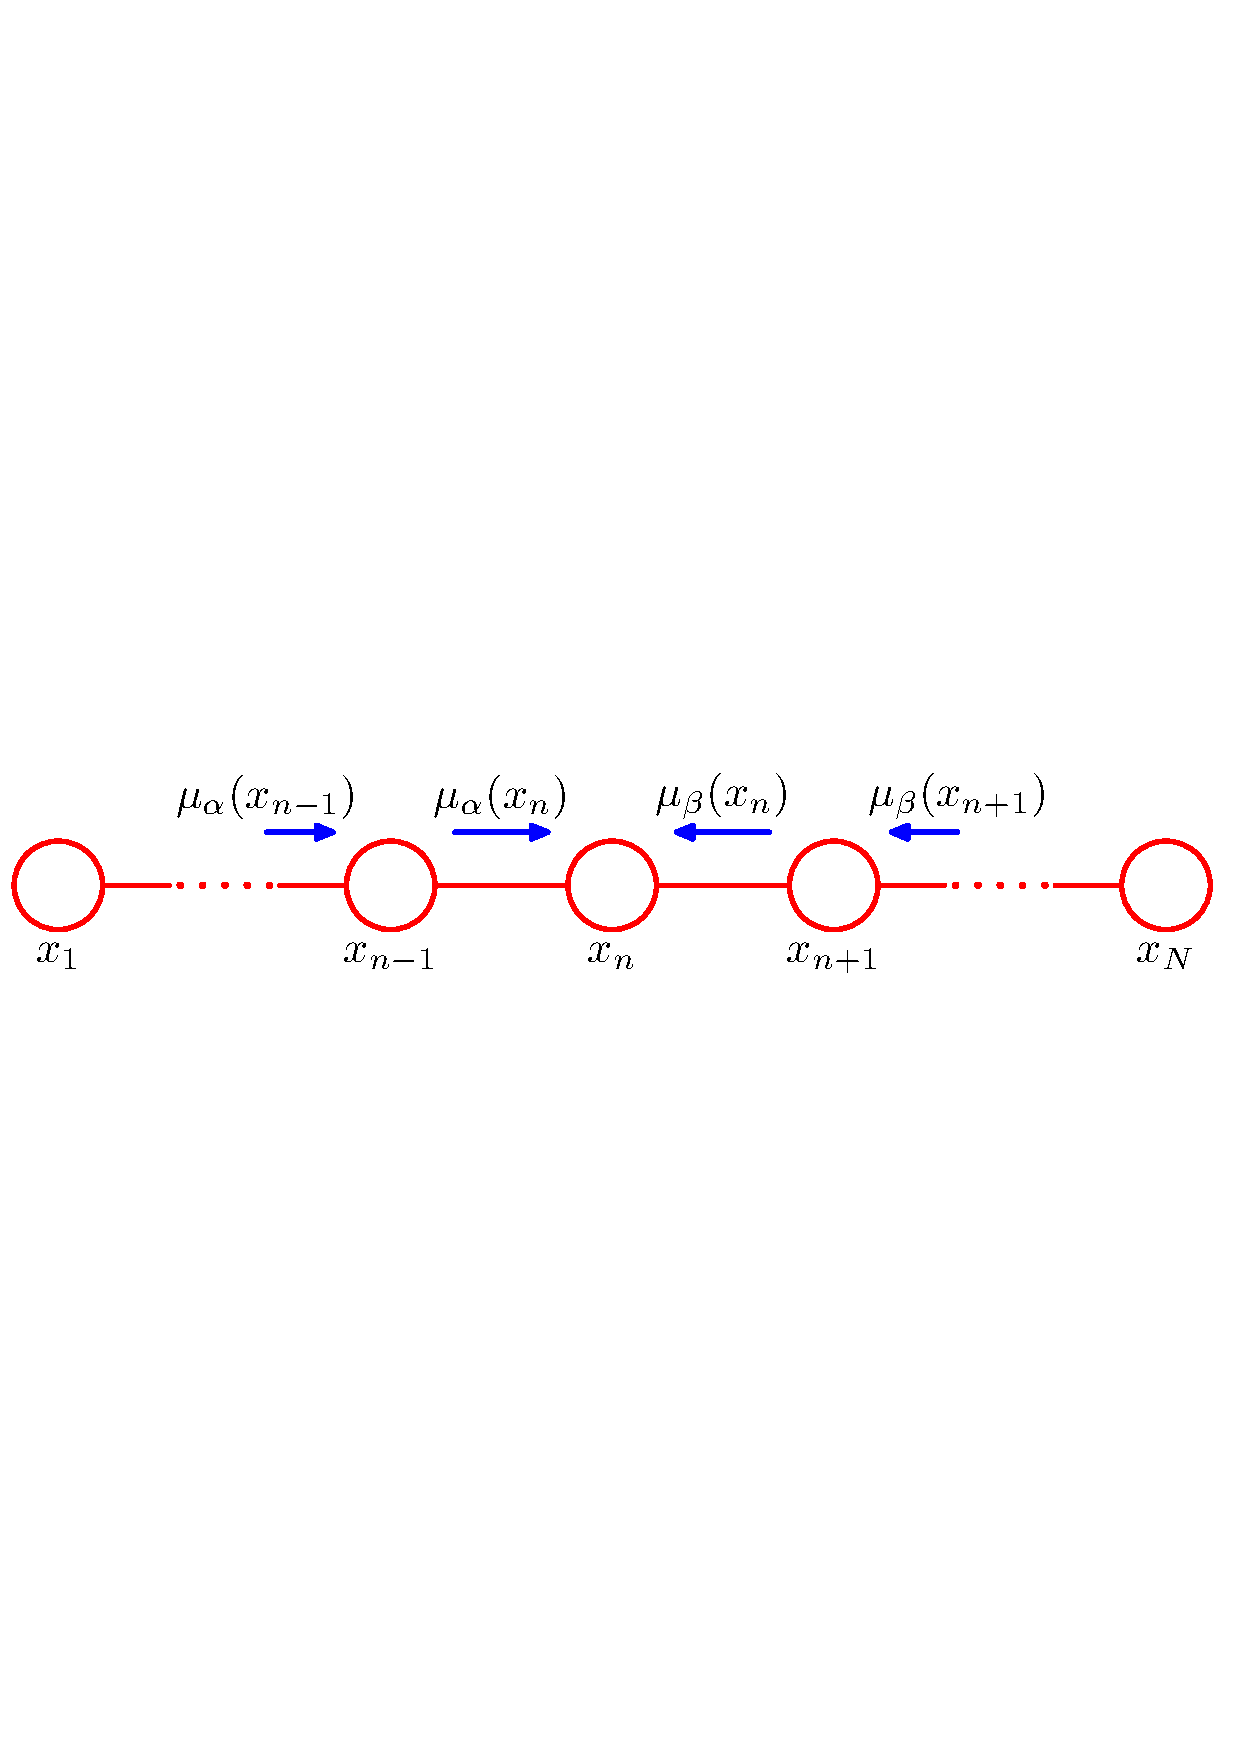
\includegraphics[width=0.5\textwidth]{figures/graphical_models_sum_product_message_passing.pdf}
		\caption{Message passing in graphical models (Bishop 8.38)}
	\end{figure}
	\item Even the normalization term $Z$ can be expressed by the messages: $Z=\sum_{x_n}\mu_{\alpha}(x_n)\mu_{\beta}(x_n)$
	\item The benefit of this recursive implementation is that we don't have to take a sum over $d$ variables ($\mathcal{O}(K^{d})$), but only have to take sums over two variables at a time ($\mathcal{O}(K^{2}d)$). Hence, the computational time scales linear with number of nodes instead exponential.
	
	Furthermore, we can share calculations between nodes, as the same messages can be re-used. Thus, calculating the marginals for all variables reduces to $\mathcal{O}(2\cdot K^2{d})=\mathcal{O}(K^2{d})$
\end{itemize}
\subsubsection{Sum-product algorithm}
\begin{itemize}
	\item The message passing idea is not limited to a Markov chain, but can be applied to any graph. For simplicity, we focus here on \textit{trees}, i.e. graphs where all nodes are connected, but without any loops/cycles, independent of the direction of the edges.
	\item In our discussion, we will focus on factor graphs as they represent the most general form of graphical models. Furthermore, cycles in MRFs can often be resolved in a factor graph so that we have less problem getting a tree-structured graph
	\item Now we will send messages from variables to factors, and from factors to variables. As a result, we get the marginalization for all variables. This algorithm is called \textbf{sum-product} algorithm as we only take sums and products
	\begin{figure}[ht!]
		\centering
		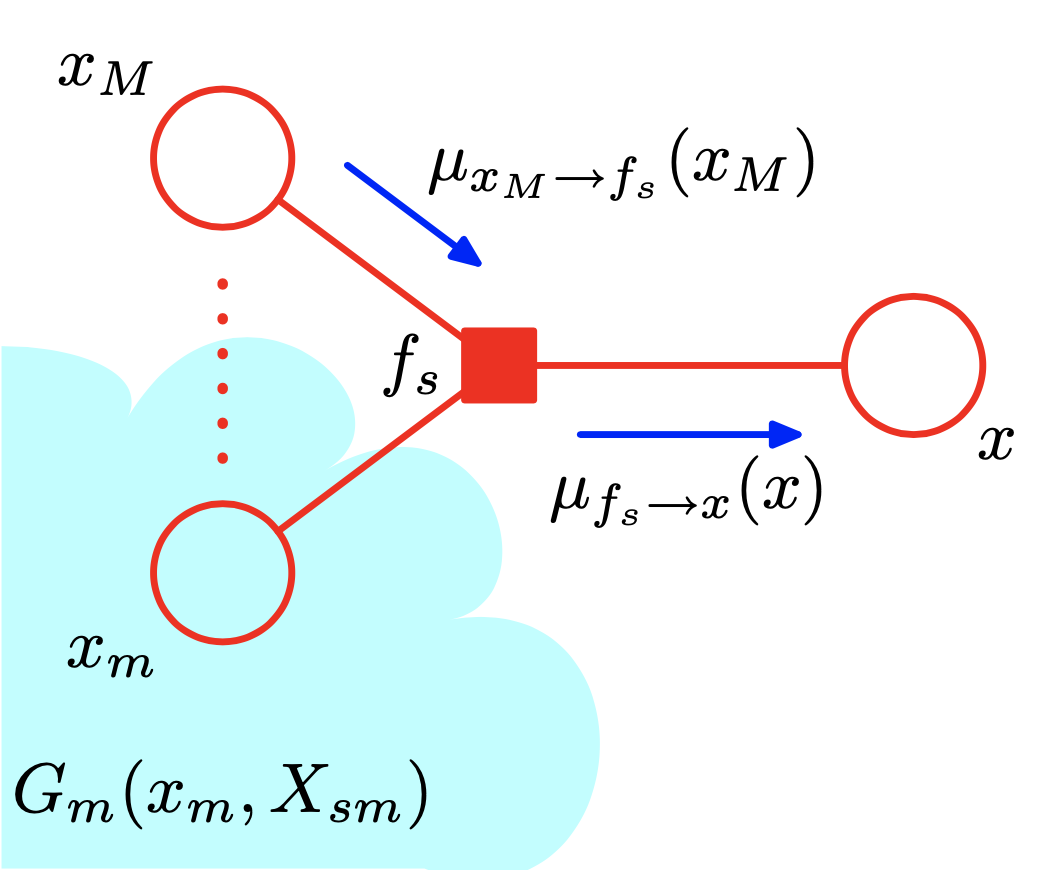
\includegraphics[width=0.2\textwidth]{figures/graphical_models_sum_product_messages_factor.png}
		\caption{Message passing to and from a factor node (Bishop 8.47)}
	\end{figure}
	\item The messages can be calculated as follows where we start at leaf nodes, and recursively go to the center of the tree:
	\begin{equation*}
	\tcbox[nobeforeafter]{\(
		\begin{split}
			\textbf{Factor$\to$Variable:} & \hspace{2mm} \mu_{\alpha\to i}(x_i)=\sum_{\bm{x}_{\alpha\setminus i}} f_{\alpha}(\bm{x}_{\alpha})\prod_{j\in \alpha\setminus i}\mu_{j\to\alpha}(x_j)\\
			& \text{If $\alpha$ leaf node:} \hspace{2mm}\mu_{\alpha\to i}(x_i)=\sum_{\bm{x}_{\alpha}} f_{\alpha}(\bm{x}_{\alpha})\\
			\textbf{Variable$\to$Factor:} & \hspace{2mm} \mu_{j\to \alpha}(x_j)=\prod_{\beta\in \text{ne}(j)\setminus \alpha}\mu_{\beta\to j}(x_j)\\
			&\text{If $j$ leaf node:} \hspace{2mm}\mu_{j\to \alpha}(x_j)=1
		\end{split}
		\)}
	\end{equation*}
	The marginalizations/beliefs are in the end:
	\begin{equation*}
	\tcbox[nobeforeafter]{\(
		\begin{split}
		\textbf{Variable belief:} & \hspace{2mm} p(x_i)=\frac{1}{Z}\prod_{\alpha\in\text{ne}(i)}\mu_{\alpha\to i}(x_i)\hspace{5mm}\text{where}\hspace{2mm}Z=\sum_{x_i}\prod_{\alpha\in\text{ne}(i)}\mu_{\alpha\to i}(x_i)\\
		\textbf{Factor belief:} & \hspace{2mm} p(\bm{x}_{\alpha})=\frac{1}{Z}f_{\alpha}(\bm{x}_\alpha) \prod_{i \in\text{ne}(\alpha)}\mu_{i \to\alpha}(x_i)\\
		\end{split}
		\)}
	\end{equation*}
	where a factor belief is the marginalization of all variables except those with an direct edge to the factor.
	\item The complexity of this algorithm scales with $\mathcal{O}(EK^{M})$ where $E$ are the number of edges, $M$ the maximum number of variables that are connected to a factor, and $K$ the maximum domain size
	\item Note that this algorithm is only exact on trees or forest (group of trees). For general graphs, we can first bring them into the shape of a tree by e.g. \textbf{variable elimination}
	\begin{itemize}
		\item Given a MRF or factor graph, we will marginalize out these variable nodes which cause a loop in our graphical model. Let's for example consider this model:
		\begin{figure}[ht!]
			\centering
			\tikz{ %
				\node[latent] (xA) {$X_A$} ; %
				\node[latent, right=of xA] (xB) {$X_B$} ; %
				\node[latent, below=of xA] (xC) {$X_C$} ; %
				\node[latent, right=of xC] (xD) {$X_D$} ; %
				\node[latent, right=of xD] (xE) {$X_E$} ; %
				
				\edge[-]{xA}{xB};
				\edge[-]{xB}{xD};
				\edge[-]{xC}{xD};
				\edge[-]{xE}{xD};
				\edge[-]{xE}{xB};
			}
		\end{figure}
		\item We can do this by simply writing down the joint probability distribution and determine a order of variables $X_1,...,X_M$ where the last variables, e.g. $X_M$, should be those which are eliminated (likely the easiest to marginalize). We then sort the sums according to the selected order.
		
		In our example, we want to eliminate $X_E$ as it has the least connections from those in the loop. The sum order is therefore:
		\begin{equation*}
			\hspace{-10mm}p(X_A,...,X_E) = \frac{1}{Z}\sum_{X_B}\sum_{X_A} \psi_{A,B}(X_A, X_B)\sum_{X_D}\psi_{B,D}(X_B, X_D) \sum_{X_C}\psi_{C,D}(X_C, X_D)\sum_{X_E} \psi_{B,E}(X_B, X_E)\psi_{D,E}(X_D, X_E)
		\end{equation*}
		\item Finally, replace the marginalized terms by a new factor, and remove node from graph. In the example, we would replace $\tau(X_B, X_D) = \sum_{X_E} \psi_{B,E}(X_B, X_E)\psi_{D,E}(X_D, X_E)$. This can be merged into the potential $\psi_{B,D}$, hence not changing the graph structure. Our final graph is a tree again, and looks as follows:
		\begin{figure}[ht!]
			\centering
			\tikz{ %
				\node[latent] (xA) {$X_A$} ; %
				\node[latent, right=of xA] (xB) {$X_B$} ; %
				\node[latent, below=of xA] (xC) {$X_C$} ; %
				\node[latent, right=of xC] (xD) {$X_D$} ; %
				
				\edge[-]{xA}{xB};
				\edge[-]{xB}{xD};
				\edge[-]{xC}{xD};
			}
		\end{figure}
	\end{itemize}
	\item The sum-product algorithm so far only calculated marginals. To set some observed variables as observed, we can use the same algorithm, but simply add additional ``hard evidence'' factor nodes, which is nothing else than a hard prior that $x_j$ has the value $\xi_j$:
	$$f_{\xi_j}(x_j)=\delta(x_j=\xi_j)$$
	Then if we apply the sum product algorithm on the extended graph again, we get the conditionals $p(x_i|x_j=\xi_j)$
\end{itemize}
\subsubsection{Max-sum algorithm}
\begin{itemize}
	\item The sum-product algorithm calculates the full marginal distribution $p(x_j)$, but sometimes, we just want to know the most likely value of $x_j$, especially if we set some variables to observed states
	\item As it turns out, we can use a very similar algorithm for this, but simply replace sums by maximum operators, and products by sums.
	\item First, let's consider what the optimum is in the general case:
	$$\bm{x}^{*}=\arg\max_{\bm{x}} \prod_{\alpha} f_{\alpha}(\bm{x}_{\alpha})$$
	where we can ignore the normalization constant. Furthermore, to simplify optimization, we can apply the log:
	$$\bm{x}^{*} = \arg\max_{\bm{x}} \sum_{\alpha} \ln f_{\alpha}(\bm{x}_{\alpha})$$
	\item Our messages passed across the graph are then as follows:
	\begin{equation*}
	\tcbox[nobeforeafter]{\(
		\begin{split}
		\textbf{Factor$\to$Variable:} & \hspace{2mm} \nu_{\alpha\to i}(x_i)=\max_{\bm{x}_{\alpha\setminus i}} \log f_{\alpha}(\bm{x}_{\alpha}) + \sum_{j\in \alpha\setminus i}\nu_{j\to\alpha}(x_j)\\
		& \text{If $\alpha$ leaf node:} \hspace{2mm}\nu_{\alpha\to i}(x_i)=\max_{\bm{x}_{\alpha\setminus i}}\log  f_{\alpha}(\bm{x}_{\alpha})\\
		\textbf{Variable$\to$Factor:} & \hspace{2mm} \nu_{j\to \alpha}(x_j)=\sum_{\beta\in \text{ne}(j)\setminus \alpha}\nu_{\beta\to j}(x_j)\\
		&\text{If $j$ leaf node:} \hspace{2mm}\nu_{j\to \alpha}(x_j)=0
		\end{split}
		\)}
	\end{equation*}
	\item The maximum beliefs/marginals are:
	\begin{equation*}
	\tcbox[nobeforeafter]{\(
		\begin{split}
		\textbf{Max-marginals:} & \hspace{2mm} q_i(x_i)=\sum_{\alpha\in\text{ne}(i)}\nu_{\alpha\to i}(x_i)\\
		\end{split}
		\)}
	\end{equation*}
	\item In the case that $q_i(x_i)$ has a unique maximum, we can simply take the argmax to get the optimum: $x^{*}_i = \arg\max_{x_i} q_i(x_i)$
	
	If this is not the case, we need to run the Viterbi algorithm (Bishop 8.4.5, we do not go in detail for this in the exam) to get the global optimum. The general idea is that some optima might depend on each other. For example, if we have something similar to a XOR, $(x_0=0, x_1=1)$ and $(x_0=1,x_1=0)$ are the optimums, but just looking at the independent marginals, $(x_0=0,x_1=0)$ and $(x_0=1,x_1=1)$ would be also optima. We can prevent this by slightly extending the messages passed around.
\end{itemize}
\newpage
\section{Variational Expectation Maximization}

\begin{itemize}
	\item The expectation maximization algorithm can be viewed from a different angle where we focus on the latent variables $z_n$
	\item For each observed data point $\bm{x}_n$, we create a latent variable $\bm{z}_n$ which \textit{explains} the observation by our underlying model
	\begin{itemize}
		\item For example, in case we have a mixture model, the latent variable $z_n$ indicates from which component $\bm{x}_n$ was created
		\item We create the model in such a way that $p(X,Z|\theta)$ can be easily calculated
	\end{itemize}
	\item As a graphical model, we can represent it as follows:
	\begin{figure}[ht!]
		\centering
		\tikz{ %
			\node[obs] (x) {$\bm{x}_n$} ; %
			\node[latent, above=of x] (z) {$\bm{z}_n$} ; %
			
			\edge{z}{x};
			
			\plate{xz}{(x)(z)}{$n=1,...,N$};
			\node[const, left=of x] (theta) {$\bm{\theta}$};
			\edge{theta}{x};
		}
	\end{figure}
	\item The objective we want to optimize is the log-likelihood $$\ln p(\bm{X}|\bm{\theta}) = \ln \left\{\sum_{\bm{Z}}p(\bm{X}, \bm{Z}|\bm{\theta})\right\}$$
	\item However, note that in the standard setting, we are not given $\bm{Z}$ so that we need to work with the posterior $p(\bm{Z}|\bm{X},\bm{\theta})$ as knowledge over latent variables. Hence, we calculate the log-likelihood under expectation of our posterior:
	$$\E_{\bm{Z}\sim p(\bm{Z}|\bm{X},\bm{\theta})}\left[\ln p(\bm{X}, \bm{Z}|\bm{\theta})\right] = \sum_{\bm{Z}} p(\bm{Z}|\bm{X},\bm{\theta}) \ln p(\bm{X}, \bm{Z}|\bm{\theta})$$
	\item As the optimization problem for the posterior and the parameters has often no analytical closed-form solution, we optimize both sequentially, leading to the general idea of the EM algorithm
	\begin{description}
		\item[E-step] Find the posterior distribution $p(\bm{Z}|\bm{X},\bm{\theta}^{\text{old}})$ where $\bm{\theta}^{\text{old}}$ means that we fix the other parameters
		\item[M-step] Optimize the log-likelihood with respect to parameters $\bm{\theta}$ while keeping the posterior fixed
		$$\bm{\theta}^{\text{new}} = \arg\max_{\bm{\theta}} \mathcal{Q}(\bm{\theta}, \bm{\theta}^{\text{old}}) = \arg\max_{\bm{\theta}} \sum_{\bm{Z}} p(\bm{Z}|\bm{X},\bm{\theta}^{\text{old}}) \ln p(\bm{X}, \bm{Z}|\bm{\theta})$$
	\end{description}
	\item In case we want to find the MAP instead of the MLE, we simply have to add the prior term $\ln p(\bm{\theta})$ to $\mathcal{Q}(\bm{\theta}, \bm{\theta}^{\text{old}})$ in the M-step 
\end{itemize}
\subsection{Generalizing EM}
\begin{itemize}
	\item We can further generalize the EM algorithm to a form, which was originally used to prove its optimization objective. 
	\item However, we can also look at it from a different perspective. It might be sometimes the case, that the posterior $p(\bm{Z}|\bm{X},\bm{\theta}^{\text{old}})$ is hard to determine. Instead, we can introduce an approximation $q(\bm{Z})$ for which we can choose the form ourselves (e.g. Gaussian, or softmax distribution over discrete states, etc.)
	\item Using this approximation, we can calculate the log likelihood by:
	\begin{equation*}
		\begin{split}
			\ln p(\bm{X}|\bm{\theta}) & = \sum_{n=1}^{N} \sum_{\bm{z}_n} q(\bm{z}_n)\ln \frac{p(\bm{x}_n, \bm{z}_n|\bm{\theta})}{p(\bm{z}_n|\bm{x}_n, \bm{\theta})}\\
			 & = \sum_{n=1}^{N} \sum_{\bm{z}_n} q(\bm{z}_n)\ln \frac{p(\bm{x}_n, \bm{z}_n|\bm{\theta})}{q(\bm{z}_n)}\frac{q(\bm{z}_n)}{p(\bm{z}_n|\bm{x}_n, \bm{\theta})}\\
			 & = \sum_{n=1}^{N} \left[\E_{q_n}\left[\log p(\bm{x}_n, \bm{z}_n|\bm{\theta})\right] + H(q_n) + \underbrace{\text{KL}\left(q_n(\bm{z}_n)||p(\bm{z}_n|\bm{x}_n, \bm{\theta})\right)}_{\geq 0}\right]\\
		\end{split}
	\end{equation*}
	\item We can define an ELBO for our objective function:
	$$\ln p(\bm{X}|\bm{\theta}) = \mathcal{L}(\bm{\theta}) \geq  \sum_{n=1}^{N} \left[\E_{q_n}\left[\log p(\bm{x}_n, \bm{z}_n|\bm{\theta})\right] + H(q_n)\right] = \mathcal{L}(\bm{\theta}, q)$$
	\item Hence, for any set of distributions $\left\{q_n(\bm{z}_n)\right\}_{n=1}^{N}$, we can define a lower bound optimization objective $\mathcal{L}(\bm{\theta}, q)$, which is equal to $\mathcal{L}(\bm{\theta})$ iff $q_n(\bm{z}_n)=p(\bm{z}_n\vert \bm{x}_n, \bm{\theta})$
	\item During the E-step, we optimize $\mathcal{L}(\bm{\theta}, q)=\ln p(\bm{X}|\bm{\theta})-\text{KL}(q||p)$ regarding $q$. As $\ln p(\bm{X}|\bm{\theta})$ is independent of $q$, we minimize the KL-divergence, meaning that we push $q_n(\bm{z}_n)$ to be similar to $p(\bm{z}_n\vert \bm{x}_n, \bm{\theta})$
	\item In the M-step, we increase $p(\bm{X}|\bm{\theta})$ by optimizing the parameters $\bm{\theta}$. Note that as $q$ is fixed in this step, the KL-divergence will increase as well, due to $q$ being now sub-optimal for the new parameters. Hence, we perform another E-step again a.s.o.
	\item Keep in mind that when optimizing $\mathcal{L}(\bm{\theta}, q)$, we need to add Lagrangian for the constraint that $q_n$ is a valid PDF:
	$$\tilde{\mathcal{L}}(\bm{\theta}, q) = \mathcal{L}(\bm{\theta}, q) + \sum_{n=1}^{N} \lambda_n \left(\sum_{\bm{z}_n} q_n(\bm{z}_n) - 1\right)$$
	Depending on our model, we might need to add additional Lagrangian to $\tilde{\mathcal{L}}(\bm{\theta}, q)$ (e.g. over $\bm{\pi}$ in mixture models)
	\item In summary, the variational EM algorithm can be summarized as follows:
	
	\begin{tcolorbox}[colback=white!85!gray,colframe=gray!75!black,title=Variational EM algorithm]
		\begin{enumerate}
			\item Choose initial $\bm{\theta}^{(0)}$
			\item Iterate until $\Delta \bm{\theta}^{(t)} < \epsilon$
			\begin{enumerate}
				\item \textbf{E-step}: Given \underline{fixed} $\bm{\theta}^{(t)}$,
				\begin{itemize}
					\item If the posterior can be determined, evaluate $q_n^{(t)}(\bm{z}_n) = p(\bm{z}_n|\bm{x}_n, \bm{\theta}^{(t)})$
					\item Otherwise, use Variational EM by increasing $\tilde{\mathcal{L}}(\bm{\theta}^{(t)}, q)$ over $q$, e.g. gradient ascend
				\end{itemize}
				\item \textbf{M-step}: Given \underline{fixed} $q^{(t)}$,
				\begin{itemize}
					\item Solve, if possible, $\bm{\theta}^{(t+1)} = \arg\max_{\bm{\theta}} \tilde{\mathcal{L}}(\bm{\theta}, q^{(t)})$ % \sum_{n=1}^{N} \E_{q_n}\left[\log p(\bm{x}_n, \bm{z}_n|\bm{\theta})\right]
					\item Otherwise, increase $\tilde{\mathcal{L}}(\bm{\theta}, q^{(t)})$ over $\bm{\theta}$, e.g. gradient ascend
				\end{itemize}
			\end{enumerate}
		\end{enumerate}
	\end{tcolorbox}
\end{itemize}
\subsubsection{Example: Mixture of multivariate Bernoulli's}
\begin{itemize}
	\item As an example, we outline the EM algorithm to optimize a mixture of multivariate Bernoulli's here. Our model distribution looks like:
	$$p(\bm{x}_n|\bm{\mu}, \bm{\pi}) = \sum_{k=1}^{K} \pi_k \prod_{i=1}^{D} \mu_{ki}^{x_{ni}} (1- \mu_{ki})^{1-x_{ni}} \hspace{4mm}\text{where}\hspace{2mm} \sum_{k=1}^{K}\pi_k = 1$$
	\item Optimizing the parameters without the EM algorithm does not has a closed-form solution because of a sum in the log:
	$$\log p(\bm{X}|\bm{\mu},\bm{\pi}) = \sum_{n=1}^{N} \log \sum_{z_n=1}^{K} \pi_{z_n} p(\bm{x}_n|\bm{\mu_{z_n}})$$
	\item Our EM objective is instead:
	\begin{equation*}
		\begin{split}
			\mathcal{L}(q,\bm{\mu}, \bm{\pi}) & = \sum_{n=1}^{N} \sum_{\bm{z}_n} q_n(\bm{z}_n) \left\{ \left(\log \pi_{z_n} + \sum_{i=1}^{D}\left[x_{ni}\log \mu_{z_n,i} + (1 - x_{ni})\log (1 - \mu_{z_n,i})\right]\right)- \log q_n(\bm{z}_n)\right\}\\
		\end{split}
	\end{equation*}
	\begin{equation*}
		\begin{split}
			\tilde{\mathcal{L}}(q,\bm{\mu}, \bm{\pi}, \lambda, \left\{\lambda_n\right\}) & = \mathcal{L}(q,\bm{\mu}, \bm{\pi}) + \lambda \left(\sum_{k=1}^{K} \pi_k - 1\right) + \sum_{n=1}^{N} \lambda_n \left(\sum_{\bm{z}_n} q_n(\bm{z}_n) - 1\right)
		\end{split}
	\end{equation*}
	\item The update equation we get by deriving $\tilde{\mathcal{L}}(q,\bm{\mu}, \bm{\pi}, \lambda, \left\{\lambda_n\right\})$ with respect to the according parameters
	\begin{description}
		\item[E-Step] Optimize $q$
		\begin{equation*}
			\begin{split}
				\frac{\partial \tilde{\mathcal{L}}}{\partial q_n(z_n)} & = \log \pi_{z_n} + \left[\sum_{i=1}^{D} x_{ni}\log \mu_{z_n,i}+(1-x_{ni})\log (1-\mu_{z_n,i})\right] - \log q_n(z_n) - 1 + \lambda_n = 0\\
				\implies q_n(z_n) & = \exp(\lambda_n-1)\pi_{z_n}\prod_{i=1}^{D} \mu_{z_n,i}^{x_{ni}}(1 - \mu_{z_n,i})^{1-x_{ni}}
			\end{split}
		\end{equation*}
		By solving for the Lagrangian $\lambda_n$, we would see that $\exp(\lambda_n-1)=1/(\sum_{z_n}q(z_n))$, and hence, being a normalization factor.
		\item[M-step] Optimize parameters $\bm{\pi}$:
		\begin{equation*}
			\begin{split}
				\frac{\partial \tilde{\mathcal{L}}}{\partial \pi_k} & = \sum_{n=1}^{N} \sum_{\bm{z}_n }  q_n(\bm{z}_n)\frac{z_{nk}}{\pi_k}  + \lambda \overset{!}{=} 0\\
				\Leftrightarrow \pi_k & = \frac{1}{\lambda} \sum_{n=1}^{N} \sum_{\bm{z}_n}  z_{nk} q_n(\bm{z}_n)\\
				\frac{\partial \tilde{\mathcal{L}}}{\partial \lambda} & = \sum_{k=1}^{K} \pi_k - 1 \overset{!}{=} 0\\
				\Leftrightarrow 1 & = \sum_{k=1}^{K} \frac{1}{\lambda} \sum_{n=1}^{N} \sum_{\bm{z}_n} z_{nk} q_n(\bm{z}_n) \\ 
				\Leftrightarrow \lambda & = \sum_{k=1}^{K} \sum_{n=1}^{N} \sum_{\bm{z}_n} z_{nk} q_n(\bm{z}_n) = \sum_{n=1}^{N} 1 = N\\
				\implies \pi_k & = \frac{\sum_{n=1}^{N} \sum_{\bm{z}_n} z_{nk} q_n(\bm{z}_n)}{N}
			\end{split}
		\end{equation*}
		Optimize parameter $\bm{\mu}$:
		\begin{equation*}
			\begin{split}
				\frac{\partial \tilde{\mathcal{L}}}{\partial \mu_{ki}} & = \sum_{n=1}^{N} q_n(k)\left[\frac{x_{ni}}{\mu_{ki}} - \frac{1-x_{ni}}{1-\mu_{ki}}\right]\\
				\implies \mu_{ki} & = \frac{\sum_{n=1}^{N} q_n(k)x_{ni}}{\sum_{n=1}^{N} q_n(k)}
			\end{split}
		\end{equation*}
	\end{description}
\end{itemize}
\subsection{Variational Inference: Variational Bayes}
\begin{itemize}
	\item In standard EM, we treat $\bm{\theta}$ to be a parameter that we want to optimize with a single value. However, looking from a Bayesian perspective, we would also treat it as a (latent) random variable and calculate its posterior, leading to the following graphical model:
	\begin{figure}[ht!]
		\centering
		\tikz{ %
			\node[obs] (x) {$\bm{x}_n$} ; %
			\node[latent, left=of x] (theta) {$\bm{\theta}$} ; %
			
			\edge{theta}{x};
			
			\plate{xz}{(x)}{$n=1,...,N$};
		}
	\end{figure}
	\item Note that we could also include latent variables $\bm{z}_n$ as in the EM algorithm, but for generality, we could simply include them in $\bm{\theta}$ as the calculations are exactly the same
	\item We perform the same derivation as for variational EM, with the difference, that $q$ is now over all parameters $\bm{\theta}$, giving us the following objective:
	\begin{equation*}
		\begin{split}
			L=\log p(X) & \geq \mathcal{L}(q)\\
			\text{where}\hspace{2mm}\mathcal{L}(q) & = \int q(\bm{\theta}) \log \left[p(X|\bm{\theta})p(\bm{\theta})\right]d\bm{\theta} - \int q(\bm{\theta})\log q(\bm{\theta})d\bm{\theta}\\
			& = \E_{q(\bm{\theta})}\left[\log \left(p(X|\bm{\theta})p(\bm{\theta})\right)\right] + H(q)
		\end{split}
	\end{equation*}
	Note that we use integrals here as parameters are often continuous.
	\item The posterior can be found by optimizing $q$:
	$$p(\bm{\theta}|\bm{X}) = \arg\max_{q(\bm{\theta})} \mathcal{L}(q)$$
	\item In practice, we restrict $q(\bm{\theta})$ to be in a function family $Q$ for  which we can calculate the maximum of $\mathcal{L}(q)$ analytically, or optimize by gradient ascend. 
	\item One example for $Q$ is to assume that all (or at least certain parts) of the parameters are independent of each other, hence:
	$$q(\bm{\theta})\in Q=\left\{\prod_{i=1}^{D}q_i(\bm{\theta}_i)\right\}$$
	where $\bm{\theta}_i$ can be either a scalar or a vector.
	\item For this case, we can simplify the objective:
	\begin{equation*}
		\begin{split}
			\tilde{L}(q) & = \int \left(\prod_{i=1}^{D} q_i(\bm{\theta}_i)\right) \log \left[p(X|\bm{\theta})p(\bm{\theta})\right]d\bm{\theta} - \sum_{i=1}^{D}\int q_i(\bm{\theta}_i)\log q_i(\bm{\theta}_i)d\bm{\theta}_i + \sum_{i=1}^{D} \lambda_i \left(\int q_i(\theta_i)d\bm{\theta}_i - 1\right)\\
			\frac{\partial \tilde{L}}{\partial q_i(\bm{\theta}_i)} & = \int \left(\prod_{j\neq i} q_j(\bm{\theta}_j)\right) \log \left[p(X|\bm{\theta})p(\bm{\theta})\right]d\bm{\theta}_{\setminus i} - \log q_i(\theta_i) - 1 + \lambda_i\\
			\Leftrightarrow q_i(\bm{\theta}_i) & = \exp\left(\lambda_i - 1\right) \exp\left\{\int \left(\prod_{i\neq j} q_j(\bm{\theta}_j)\right)\log \left(p(\bm{X}|\bm{\theta})p(\bm{\theta})\right) \right\}\\
		\end{split}
	\end{equation*}
	\item Hence, our approximated posterior over $\bm{\theta}_i$ is the expectation of $\log p(X,\bm{\theta})$ over all other parameters:
	\begin{equation*}
		\tcbox[nobeforeafter]{\(p(\bm{\theta}|\bm{X})=\prod_{i=1}^{D}q_i(\bm{\theta}_i), \hspace{2mm}q_i(\bm{\theta}_i) = \frac{1}{Z} \exp\left(\E_{q_{\setminus i}}\left[\log p(\bm{X}, \bm{\theta})\right]\right)\)}
	\end{equation*}
	We iterate this update for each $q$ until convergence.
	\item Note that Variational Bayes is highly related to Gibbs sampling as there, we do not calculate the full probability distribution $q$, but simply alternate between sampling from the different $q_i$'s. By iterating until convergence/for a sufficient number of time, we also reach the true posteriors.
	
\end{itemize}
\subsubsection{Example: Gaussian with mean and variance as latent variables}
\begin{itemize}
	\item We consider the following graphical model:\\
	\begin{figure}[ht!]
		\centering
		\tikz{ %
			\node[obs] (x) {$x_n$} ; %
			\node[latent, above=of x] (mu) {$\mu$} ; %
			\node[latent, right=of mu] (tau) {$\tau$} ; %
			
			\edge{mu}{x};
			\edge{tau}{x};
			\edge{tau}{mu};
			
			\plate{xz}{(x)}{$n=1,...,N$};
		}
	\end{figure}

	where
	\begin{equation*}
		\begin{split}
			p(\bm{X}|\mu, \tau) & = \prod_{n=1}^{N} \mathcal{N}(x_n|\mu, \tau^{-1})\\
			p(\tau) & = \text{Gamma}(\tau|a_0, b_0)\\
			p(\mu|\tau) & = \mathcal{N}(\mu|\mu_0, (\lambda_0 \tau)^{-1})
		\end{split}
	\end{equation*}
	\item Now, let's assume that we approximate the posteriors by $q(\tau, \mu)=q(\tau)q(\mu)$. Our objective (excluding the Lagrangian) is:
	$$\mathcal{L}(q_{\mu}, q_{\tau}) = \int q_{\mu}(\mu)q_{\tau}(\tau)\left[\log p(\bm{X}|\mu, \tau)p(\mu|\tau)p(\tau)\right] + H(q_{\mu}) + H(q_{\tau})$$
	\item When solving this, we will end up with:
	\begin{equation*}
		\begin{split}
			q_{\mu}(\mu) & = \mathcal{N}\left(\mu\Big\vert \frac{\lambda_0\mu_0 + N\overline{x}}{\lambda_0 + N}, \left[(\lambda_0 + N)\E_{q_{\tau}}[\tau]\right]^{-1}\right)\\
			q_{\tau}(\tau) & = \text{Gamma}\left(\tau\Big\vert a_0 + \frac{N}{2}, b_0 + \frac{1}{2}\E_{q_{\mu}}\left[\sum_n (x_n-\mu)^2+\lambda_0(\mu-\mu_0)^2\right]\right)\\
			\Rightarrow p(\mu, \tau|\bm{X}) &\approx q_{\mu}(\mu)q_{\tau}(\tau)
		\end{split}
	\end{equation*}
\end{itemize}
\subsubsection{Combining Variational EM and Variational Bayes}
\begin{itemize}
	\item The Variational EM algorithm and the variational Bayes are strongly related. In fact, we can generalize the framework to combine both of them
	\item Our goal is to optimize the parameters $\bm{\theta}$, and marginalize over latent variables $\bm{Z}$, leading to the objective:
	$$\ln p(\bm{X}) = \E_{q(\bm{Z}, \bm{\theta})}\left[\ln p(\bm{X}, \bm{Z}, \bm{\theta})\right] + \underbrace{H(q_Z) + H(q_{\theta})}_{\text{assume } q(\bm{Z},\bm{\theta})=q_Z(\bm{Z})q_{\theta}(\bm{\theta})} + \underbrace{\text{KL}\left(q_Z q_{\theta} || p(\bm{Z}, \bm{\theta}|\bm{X})\right)}_{\geq 0}$$
	\item Again, we can optimize an ELBO instead:
	$$\ln p(\bm{X}) \geq \E_{q_Z q_{\theta}}\left[\ln p(\bm{X}, \bm{Z}, \bm{\theta})\right] = \mathcal{L}(q_Z, q_{\theta})$$
	\item Assuming $\tilde{\mathcal{L}}(q_Z, q_{\theta})$ being the objective function including the Lagrangian, we have the following steps:
	\begin{description}
		\item[$\E_{Z}$-step]: $\max_{q_Z} \tilde{\mathcal{L}}(q_Z, q_{\theta})$
		\item[$\E_{\theta}$-step]: $\max_{q_{\theta}} \tilde{\mathcal{L}}(q_Z, q_{\theta})$
	\end{description}
	\item As this is a generalization, we can find both the EM algorithm and variational Bayes in it. The EM algorithm is found if we choose $q_{\theta}(\theta)=\delta(\theta'-\theta)$, where $\theta'$ is optimized $\Rightarrow$ equal to replacing $q_{\theta}$ with MLE/MAP solution
	\item For variational Bayes, we can simply ignore the $Z$ part as we fully focus on $q_{\theta}$. The iteration over the $\E_{\theta}$-step is equal to variational Bayes
\end{itemize}
\subsection{Variational Auto-Encoder (VAE)}
\begin{itemize}
	\item One implementation with neural networks of this variational framework are VAEs, where we model the likelihood by:
	$$p(\bm{X}, \bm{Z}|\bm{\theta}) = \underbrace{p(\bm{X}|\bm{Z}, \bm{\theta}_2)}_{\text{decoder}}\underbrace{p(\bm{Z}|\bm{\theta}_1)}_{\text{encoder/prior}}$$
	\item The aim is to find a lower-dimensional representation $Z$ of the data $X$ (\textit{encode} $X$). For approximating the posterior, we use again $q(\bm{Z}|\bm{X},\bm{\lambda})\approx p(\bm{Z}|\bm{X}, \bm{\theta}_1, \bm{\theta}_2)$, where $q$ is now a neural network
	\item As a prior distribution, we use e.g. $p(\bm{Z}|\bm{\theta}_1) \sim \mathcal{N}(0,1)$ which encourages the latents to be independent. Furthermore, by using this prior, we can treat VAEs as a non-linear version of PCA (in case we choose student-t distribution, we would get non-linear ICA)
	\item Optimize the ELBO of the log-likelihood via SGD:
	\begin{equation*}
		\begin{split}
			\mathcal{L}(\bm{\theta}) & = \ln p(\bm{X}|\bm{\theta}) = \ln \int p(\bm{X}|\bm{Z},\bm{\theta})p(\bm{Z}|\bm{\theta})d\bm{Z}\\
			\mathcal{L}(\bm{\theta}, \bm{\lambda}) & = \E_{q(Z|X,\lambda)}\left[\ln p(\bm{X}|\bm{Z},\bm{\theta}_2) + \ln p(\bm{Z}|\bm{\theta}_1)\right] + H(q(\bm{Z}|\bm{X}, \bm{\lambda}))
		\end{split}
	\end{equation*}
	\item To prevent the integral, we can sample instead. To make these samples differentiable, we need to use the reparameterization trick:
	\begin{equation*}
		\begin{split}
			z^{(k)}\sim q(z|x, \lambda) & \Rightarrow z=g_{\lambda}(x, \epsilon), \epsilon\sim p(\epsilon)
		\end{split}
	\end{equation*}
	As for a multivariate Gaussian with diagonal covariance, we have $g_{\lambda}(\bm{x}, \bm{\epsilon})=\bm{\mu}_{\lambda}(x)+\bm{\sigma}_{\lambda}\odot \bm{\epsilon}, \epsilon\sim\mathcal{N}(0,1)$
\end{itemize}
\newpage
\section{Sampling methods}
\begin{itemize}
	\item In the previous chapter, we have seen that we can perform inference by approximating the posterior distribution. However, as alternative, we can also consider Monte Carlo techniques, i.e. sampling
	\item In most practical cases, we often want to evaluate expectations over the posterior. This we can approximate by an average over samples:
	$$\E_{p(\bm{x})}\left[f(\bm{x})\right] \approx \frac{1}{N}\sum_{n=1}^{N} f(\bm{x}_n), \hspace{2mm} \bm{x}_n\sim p(\bm{x})$$
	This can be for example used for prediction:
	$$p(y^{*}|x^{*}) = \int p(y^{*}\vert x^{*}, \bm{\theta})p(\bm{\theta}|\bm{X}, \bm{Y})d\bm{\theta} = \E_{p(\bm{\theta}|\bm{X}, \bm{Y})}\left[p(y^{*}\vert x^{*}, \bm{\theta})\right] \approx \frac{1}{K}\sum_{k=1}^{K} p(y^{*}\vert x^{*}, \bm{\theta}^{(k)}), \hspace{2mm} \bm{\theta}^{(k)}\sim p(\bm{\theta}|\bm{X}, \bm{Y})$$
	\item Hence, we will look at different techniques for sampling from more complex distributions than standard Gaussians
\end{itemize}
\subsection{Regular Sampling}
\begin{itemize}
	\item As an introduction, we look at how we can sample from simple, known distributions, and verify the correctness of the Monte Carlo approximation
	\item Assume we draw $N$ samples from $p(z)$: $z_i\sim p(z)$, $i=1,...,N$
	\item We can calculate $\E\left[f\right]\approx \widehat{E\left[f\right]}=\left<f\right> = \frac{1}{N}\sum_{n=1}^{N}f(z_i)$ for approximating the expectation. Note that we introduced here the different notations for the Monte Carlo approximation
	\item To verify that our approximation makes sense, we first check whether we have an \textit{unbiased} estimator:
	$$\E\left[\left<f\right>\right] = \E\left[\frac{1}{N}\sum_{i=1}^{N}f(z_i)\right]=\frac{1}{N}\sum_{i=1}^{N}\E\left[f(z_i)\right]=\E\left[f(z)\right]$$
	\item Furthermore, we would like that with an infinite amount of samples, our variance goes to zero:
	$$\mathbb{V}\text{ar}\left[\left<f\right>\right]=\frac{1}{N^2}\sum_{i=1}^{N}\mathbb{V}\text{ar}\left[f(z_i)\right] = \frac{1}{N}\mathbb{V}\text{ar}\left[f\right]$$
	Hence, with $N\to\infty$, we linearly reduce the variance compared to a single sample.
	\item As a last part, we will look into how we can sample from any \textit{known} distribution, given a uniform sampler
	\begin{description}
		\item[Discrete random variables]  In case of a discrete random variable $z\in\left\{1,2,...,K\right\}$, and given the distribution $p(z)$, we first have to calculate the cumulative density function: $p(z\leq \zeta)$. Then, given $u_i\sim U(0,1)$, the sample $k$ of $p(z)$ is where $p(z\leq k-1)\leq  u_i < p(z\leq k)$
		\item[Continuous random variables] For continuous variables, we need to calculate the CDF by an integral:
		$$F(\zeta)=\int_{-\infty}^{\zeta} p(z)dz = p(z\leq \zeta)$$
		, and take its inverse $F^{-1}$. Then, given $u_i\sim U(0,1)$, our sample is $z_i=F^{-1}(u_i)$ which is a change of variables.
	\end{description}
\end{itemize}
\subsection{Rejection sampling}
\begin{itemize}
	\item Assume we have a probability density $p(z)$ from which we want to sample. Choose another distribution $q(z)$, called \textit{proposal} distribution, from which we can sample. Further constraints are that the unnormalized distributions $\tilde{p}(z)\propto p(z), \tilde{q}(z)\propto q(z)$ fulfill:
	$$\int \tilde{q}(z)dz < \infty, \tilde{p}(z)\leq \tilde{q}(z) \forall z$$
	\item Now, we can generate samples from $p(z)$ by a simple algorithm:
	\begin{tcolorbox}[colback=white!80!gray,colframe=gray!75!black,title=Pseudocode for rejection sampling]
		\begin{algorithm}[H]
			\SetAlgoLined
			\For{$n=1,...,N$}{
				\While{No sample for $z_n$ accepted}{
					Sample $\hat{z}$ from $q(z)$\;
					Sample $u\sim U(0,1)$\;
					\eIf{$u<\frac{\tilde{p}(\hat{z})}{\tilde{q}(\hat{z})}$}{Accept sample $z_n=\hat{z}$\;}{Reject sample $\hat{z}$ and re-sample\;}
				}
			}
			Return samples $\left\{z_n\right\}_{n=1}^{N}$\;
		\end{algorithm}
	\end{tcolorbox}
	\item The principle of rejection sampling is visualized in Figure~\ref{fig:sampling_rejection_sampling}
	\begin{figure}[ht!]
		\centering
		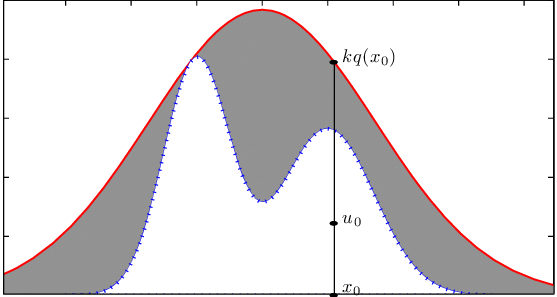
\includegraphics[width=0.3\textwidth]{figures/sampling_rejection_sampling.png}
		\caption{Visualizing rejection sampling. In the figure, $\tilde{q}(z)$ is denoted as $kq(z)$, and $x_0$ is the initial sample from $q$.}
		\label{fig:sampling_rejection_sampling}
	\end{figure}
	\item To show that we actually generate samples from $p(z)$, we can write down the probability for a value $z_i$ to be picked. First, the chance of $z_i$ being generated in first place is $q(z_i)$. Next, the chance of $z_i$ being accepted, is $\frac{\tilde{p}(z_i)}{\tilde{q}(z_i)}$. Together, we get the probability of $z_i$:
	$$\hat{p}(z_i) = q_(z_i)\frac{\tilde{p}(z_i)}{\tilde{q}(z_i)} \propto p(z_i)$$
	Hence, we actually generate samples from $z_i$ although we initially sample from $q(z)$
	\item One requirement of rejection sampling to work well is that the area between $\tilde{p}(z)$ and $\tilde{q}(z)$ is small. The efficience of this sampler can be measured by the acceptance rate, which is $\E_{z_i\sim q}\left[\frac{\tilde{p}(z_i)}{\tilde{q}(z_i)} \right]$. If this value is low, it means that a lot of samples are rejected, hence the sampling process takes longer. This gets especially critical in higher dimensions as we need to make sure that \textit{for all} $z_i$, $\tilde{q}(z_i)$ is greater than $\tilde{p}(z_i)$. Finding a simple distribution in high dimensions that fulfills this requirement is often not trivial
\end{itemize}
\subsection{Importance sampling}
\begin{itemize}
	\item Another approach for estimating an expectation is not generating actual samples from $p$, but simply weight samples by their \textit{importance}
	\item Again, we need two distributions: $p$ over which we want to determine the expectation, and $q$ that we actually sample from. Note that for this algorithm to work, none of these distributions need to be normalized. The only thing that is required is that we can sample from the normalized density of $q$.
	\item The pseudo-code for the importance sampling is fairly simple and straight forward: \begin{tcolorbox}[colback=white!80!gray,colframe=gray!75!black,title=Pseudocode for importance sampling]
		\begin{algorithm}[H]
			\SetAlgoLined
			Sample $\left\{z_n\right\}_{n=1}^{N}$ from $q(z)$\;
			Calculate the weights $w_n=\frac{p(z_n)}{q(z_n)}$\;
			Determine expectation by $\E_p[f]\approx \frac{\sum_n w_n f(z_n)}{
			\sum_n w_n}$\;
		\end{algorithm}
	\end{tcolorbox}
	\item The intuition of importance sampling can be shown when plugging in the two distributions:
	$$\E_p[f]=\int p(z)f(z)dz=\frac{\int q(z)\frac{p(z)}{q(z)}f(z)dz}{\underbrace{\int q(z)\frac{p(z)}{q(z)}dz}_{=1}} = \frac{\E_q\left[w_z\cdot f(z)\right]}{\E_q\left[w_z\right]} \approx \E_q\left[\frac{\sum_i w_i f(z_i)}{\sum_i w_i}\right]$$
	\item Although importance sampling can use all samples, it has two major drawbacks:
	\begin{itemize}
		\item The estimate of $\E[f]$ is \underline{not} unbiased. Imagine we would sample only a single time ($N=1$ in pseudo code). As the sum drops out, we end up with $f(z_i)$ where $z_i$ is sampled from $q$, and not $p$! This bias decreases with the number of samples, but should always be kept in mind as an accurate estimate might require more samples, especially when it occurs with the second drawback.
		\item The importance weighting estimate has a high variance when if $p$ differs strongly from $q$, especially when $p(z_i)\gg q(z_i)$ as the weight is very high for this data point. Imagine $q$ is a Gaussian with a large variance, while $p$ is a peaked Gaussian around 0. For most of the samples, $p(z)\ll q(z)$, and hence their weight is low. But for a small of points, namely close to 0, $p(z)$ is much greater than $q(z)$ resulting in a high weight. If we now sample e.g. 100 times, all points except those around 0 are neglected due to their low weight. And as those important points are rarely sampled from $q$, we need many samples to reduce the variance. This problem occurs even stronger in high-dimensional spaces.
	\end{itemize}
	\item Furthermore, not that importance sampling can only be used for approximating an expectation, and not for generating independent samples from $p$
\end{itemize}
\subsection{Ancestral Sampling}
\begin{itemize}
	\item Assume we have given a Bayesian network, and want to sample from the joint probability. We can write the joint probability as:
	$$p(\bm{z})=\prod_{i=1}^{d} p(z_i\vert z_{\text{pa}(i)})$$
	where we use a topological ordering $z_1,...,z_d$ with $z_j<z_i$ if $j\in \text{pa}(i)$
	\item Now we can simply sample by sampling from each of the conditionals, in the topological ordering. For example, assume we have the following Bayesian network:
	
	\begin{figure}[ht!]
		\centering
		\tikz{ %
			\node[latent] (z1) {$z_1$} ; %
			\node[latent, right=of z1] (z3) {$z_3$} ; %
			\node[latent, above=of z3] (z2) {$z_2$} ; %
			\node[latent, below=of z3] (z4) {$z_4$} ; %
			\node[latent, right=of z2] (z5) {$z_5$} ; %
			\node[latent, right=of z4] (z6) {$z_6$} ; %
			
			\edge{z1}{z2};
			\edge{z1}{z3};
			\edge{z1}{z4};
			\edge{z2}{z5};
			\edge{z3}{z5};
			\edge{z3}{z6};
			\edge{z2}{z6};
			\edge{z4}{z6};
		}
	\end{figure}

	Then we can sample as follows:
	\begin{equation*}
		\begin{split}
			\tilde{z}_1 & \sim p(z_1)\\
			\tilde{z}_2 & \sim p(z_2|z_1=\tilde{z}_1)\\
			\tilde{z}_3 & \sim p(z_3|z_1=\tilde{z}_1)\\
			\tilde{z}_4 & \sim p(z_4|z_1=\tilde{z}_1)\\
			\tilde{z}_5 & \sim p(z_5|z_2=\tilde{z}_2,z_3=\tilde{z}_3)\\
			\tilde{z}_6 & \sim p(z_6|z_2=\tilde{z}_2,z_3=\tilde{z}_3,z_4=\tilde{z}_4)\\
		\end{split}
	\end{equation*}
	
	\item Note that for sampling from each of the individual distributions, we can use the other techniques like rejection or importance sampling. 
	
	% \item \TODO{Question: lecture notes say that it works badly with high dimensions, but other sources say it works well. Why would it not work in high dimensions?}
\end{itemize}
\subsection{Markov-Chain Monte Carlo}
\begin{itemize}
	\item Given a target distribution $p(x)$ that we want to sample from, we setup a Markov chain such that $p(x_n)\to p(x)$ as $N\to\infty$, i.e. such that $p(x)$ is its equilibrium distribution
	
	\begin{figure}[ht!]
		\centering
		\tikz{ %
			\node[latent] (x1) {$x_1$} ; %
			\node[latent, right=of x1] (x2) {$x_2$} ; %
			\node[latent, right=of x2] (x3) {$x_3$} ; %
			\node[const, right=of x3] (xetc1) { \hspace{2mm}...\hspace{2mm} } ; %
			\node[latent, right=of xetc1] (xN) {$x_N$} ; %
			\node[const, right=of xN] (xetc2) { \hspace{2mm}...\hspace{2mm} } ; %
			\node[latent, right=of xetc2] (xInfty) {$x_{\infty}$} ; %
			
			\edge{x1}{x2};
			\edge{x2}{x3};
			\edge{x3}{xetc1};
			\edge{xetc1}{xN};
			\edge{xN}{xetc2};
			\edge{xetc2}{xInfty};
		}
	\end{figure}
	\item Note that as MCMC runs ancestral sampling on a chain, two consecutive samples are no longer independent. Still, we can assume that the dependency between two fairly distant samples is neglectable
	\item We start sampling $x_1$ from an initial distribution $q(x_1)$ which can be chosen arbitrarily (but the closer $q$ to $p$, the faster the convergence and hence, faster sampling). For the next samples, we use a \underline{transition kernel} $T$ to get $x_2\sim T(x_2|x_1)$
	\item The transition kernel is usually independent of time (most efficient), but can be extended to multiple steps (e.g. $x_t$ is sampled by $T_1$, $x_{t+1}$ from $T_2$, and $x_{t+2}$ again from $T_1$)
	\item The marginal distribution can be determined by:
	$$q(x_{n}) = \int q(x_{n-1})T(x_{n}|x_{n-1})dx_{n-1}$$
	and the joint probability for all $x_1,...,x_N$ is:
	$$q(x_1,...,x_N) = q(x_1)\prod_{i=2}^{N}T(x_i|x_{i-1})$$
	\item The equilibrium is reached when $x_N\sim p(x)$ (i.e. $p(x)$ is an invariant of the chain):
	$$p(x_{N+1}) = \int T(x_{N+1}|x_N)p(x_N)dx_N$$ 
	In this case, $p(x)$ is called to be an invariant of the chain. Note that a chain can have multiple invariants, as if $T$ is the identity transformation, any distribution is an invariant of that chain
	\item A sufficient but not necessary condition of an invariant $p(x)$ is that it satisfies the property of \underline{detailed balance}:
	$$p(x_t)T(x_{t+1}|x_t) = p(x_{t+1})T(x_t|x_{t+1})$$
	This property can be interpreted as the Markov chain being reversible. Although detailed balance is not required, it is mostly easier to fulfill when designing a kernel
	\item Another property we are looking for is \underline{ergodicity}. A sufficient condition for ergodicity is that any state $x_N$ has a positive probability, for any $N$.
	\item If we have an ergodic Markov chain and $p^{\star}(x)$ being an invariant, then $p^{\star}(x)$ is a unique equilibrium, where for any start distribution $q(x_0)$, the distribution $q(x_N)$ with $N\to\infty$ converges to the required distribution $p^{\star}(x)$.
	\item The sketch of the sampling process is:
	
	\begin{algorithm}[H]
		Sample initial state $x_0$ from $q(x_0)$\;
		\For{$t=0,...,N$}{
			Sample $x_{t+1}\sim T(x_{t+1}|x_{t})$\;
		}
		Output $x_N$ as sample of $p^{\star}(x)$\;
	\end{algorithm}
	$N$ has to be large enough in this case, and is often referred to as \textit{burn-in} time. 
	
	In addition, note that the required $N$ can be reduced by reducing the distance between $q$ and $p$. Thus, for generating multiple samples, we can take the first sample $x_N$, and continue the chain for additional $M$ steps, where usually $M\ll N$ (but $M$ must be certain size to guarantee independence of samples, depends on $T$). Then, $x_{N+M}$ is a new sample from $p$.
	
	\item The problem of MCMC is how we can find the transition kernel $T$ for a distribution $p$. Once we have found two kernels, we can combine those to new kernels:
	\begin{equation*}
		\begin{split}
			T_3 & = \alpha T_1 + (1 - \alpha) T_2, \hspace{2mm}(\alpha \in [0,1])\\
			T_3 & = T_2 \circ T_1 \hspace{5mm}(\text{composition, first apply $T_1$, then $T_2$})
		\end{split}
	\end{equation*}
	\item One way to overcome this problem is the Metropolis-Hastings algorithm, which uses a form of rejection sampling to allow any transition kernel $T$
\end{itemize}
\subsubsection{Metropolis-Hastings algorithm}
\begin{itemize}
	\item Choose a proposal transition kernel $Q(x_{t+1}|x_{t})$ (e.g. a random walk). Then we can sample from $p^{\star}(x)$ as follows:
	\begin{tcolorbox}[colback=white!80!gray,colframe=gray!75!black,title=Pseudocode for Metropolis-Hastings algorithm]
		\begin{algorithm}[H]
			\SetAlgoLined
			Sample initial state $x_0$ from $q(x_0)$\;
			\For{$t=0,...,N$}{
				Sample $\tilde{x}_{t+1}\sim Q(\tilde{x}_{t+1}|x_{t})$\;
				Compute acceptance probability $\alpha(\tilde{x}_{t+1}|x_t) = \min\left(1, \frac{p^{\star}(\tilde{x}_{t+1}) Q(x_t|\tilde{x}_{t+1})}{p^{\star}(x_t)Q(\tilde{x}_{t+1}|x_{t})}\right)$\;
				Sample $u_t\sim U(0,1)$\;
				\eIf{$u_t \leq \alpha(\tilde{x}_{t+1}|x_t) $}{accept sample $x_{t+1}=\tilde{x}_{t+1}$\;}{reject sample and stay at current state: $x_{t+1}=x_t$\;}
			}
			Output $x_N$ as sample of $p^{\star}(x)$\;
		\end{algorithm}
	\end{tcolorbox}	
	We can view the combination of $Q$ and acceptance probability $\alpha$ as our transition kernel $T=\alpha\circ Q$.
	\item Given this simple algorithm, we can design the transition kernel $Q$ with minimal knowledge of $p^{\star}$. For example, a kernel which mostly works well is to combine larger and smaller random walk steps. This can be very helpful in high-dimensional space as it can explore in different scales, and hence, in contrast to rejection and importance sampling, still works well in high dimensions
	\item Nonetheless, keep in mind that the performance now depends on the transition kernel $Q$. If it is designed poorly, many samples are rejected and we again end up with an inefficient sampling process. For example, if we have a highly multi-modal distribution, we need to have large enough steps to be able to jump between modes. But as said before, this is much less knowledge we need of $p^{\star}$ compared to the other discussed sampling algorithms
	\item We can sketch the proof here for the detailed balance. If a new sample $x_{t+1}$ is accepted, it has the probability:
	\begin{equation*}
		\begin{split}
			p^{\star}(x_t)T(x_{t+1}|x_{t}) & = p^{\star}(x_t)Q(x_{t+1}|x_{t})\min\left(1, \frac{p^{\star}(x_{t+1}) Q(x_t|x_{t+1})}{p^{\star}(x_t)Q(x_{t+1}|x_{t})}\right)\\
			& = \min\left(p^{\star}(x_t)Q(x_{t+1}|x_{t}), p^{\star}(x_{t+1}) Q(x_t|x_{t+1})\right)\\
			& = p^{\star}(x_{t+1})Q(x_{t}|x_{t+1})\min\left(1, \frac{p^{\star}(x_{t}) Q(x_{t+1}|x_{t})}{p^{\star}(x_{t+1})Q(x_{t}|x_{t+1})}\right)\\
			& = p^{\star}(x_{t+1})T(x_{t}|x_{t+1})
		\end{split}
	\end{equation*}
	As we can interchange $x_t$ and $x_{t+1}$, $p^{\star}$ is an invariant of the Markov chain.
	
	In case $\tilde{x}_{t+1}$ was rejected, we stay at $x_t$ which satisfies the detailed balance anyways.
\end{itemize}
\subsubsection{Gibbs sampling}
\begin{itemize}
	\item Gibbs sampling is a special case of the Metropolis-Hastings algorithm, where the acceptance probability is always 1. The idea is that we cannot easily sample from a big joint distribution, but sampling a single variable given all others is feasible/much simpler. 
	\item Hence, we sample a D-dimensional vector $(x_1,x_2,...,x_D)$ by sampling from the conditional distributions of a single variable $x_i$ where we keep all other variables fixed. In pseudo-code, we can define Gibbs sampling as:
	\begin{tcolorbox}[colback=white!80!gray,colframe=gray!75!black,title=Pseudocode for Gibbs sampling]
		\begin{algorithm}[H]
			\SetAlgoLined
			Choose an initial state $\left\{x_i:i=1,...,M\right\}$\;
			\For{$t=0,...,N$}{
				Sample $x_1^{(t+1)}\sim p(x_1|x_2^{(t)}, x_3^{(t)},...,x_M^{(t)})$\;
				Sample $x_2^{(t+1)}\sim p(x_2|x_1^{(t+1)}, x_3^{(t)},...,x_M^{(t)})$\;
				... \\
				Sample $x_M^{(t+1)}\sim p(x_M|x_2^{(t+1)}, x_3^{(t+1)},...,x_{M-1}^{(t+1)})$\;
			}
			Output $\left\{x_1^{(N)},...,x_M^{(N)}\right\}$ as sample of $p(x_1,...,x_M)$\;
		\end{algorithm}
	\end{tcolorbox}	
	\item Clearly, $p(\bm{x})$ is an invariant of the Markov chain because at each step, we sample from the correct conditional $p(x_i,\bm{x}_{\setminus i})$. But note that detailed balance can only be guaranteed if the order of $x_i$'s is randomized every iteration.
	\item For ergodicity, we just need to make sure that the conditionals are not zero for any point. Otherwise, we have to prove ergodicity explicitly.
	\item The acceptance probability of a sample according to the Metropolis-Hastings algorithm is in case of Gibbs sampling:
	$$\alpha(\bm{x}^{(t+1)}|\bm{x}^{(t)}) = \frac{p^{\star}(\bm{x}^{(t+1)}) Q(\bm{x}^{(t)}|\bm{x}^{(t+1)})}{p^{\star}(\bm{x}^{(t)})Q(\bm{x}^{(t+1)}|\bm{x}^{(t)})} = \frac{p^{\star}(x_i^{(t+1)}|\bm{x}_{\setminus i}^{(t+1)})p^{\star}(\bm{x}_{\setminus i}^{(t+1)})\cdot p^{\star}(x_i^{(t)}|\bm{x}_{\setminus i}^{(t+1)})}{p^{\star}(x_i^{(t)}|\bm{x}_{\setminus i}^{(t)})p^{\star}(\bm{x}_{\setminus i}^{(t)})\cdot p^{\star}(x_i^{(t+1)}|\bm{x}_{\setminus i}^{(t)})} = 1$$
	where $\bm{x}_{\setminus i}^{(t)}=\bm{x}_{\setminus i}^{(t+1)}$ as the other variables do not change.
\end{itemize}
\newpage
\section{Sequential Data}
\begin{itemize}
	\item Most models we discussed so far assumed that multiple data points $\bm{x}_n$ are independent of each other. However, in many use-cases, we have e.g. temporal data where consecutive data points dependent on each other
	\item The likelihood of such data can be written as:
	$$p(x_1,...,x_N) = \prod_{n=1}^{N} p(x_n|x_1,...,x_{n-1})$$
	\item Here, we will focus on Markov models and its different variations
\end{itemize}
\subsection{Markov models}
\begin{itemize}
	\item One of the simplest models for sequential data are Markov models, where we limit the conditionals to a fixed size. For example, a \textit{first-order} Markov model has the likelihood $p(x_1)\prod_{n=2}^{N}p(x_n|x_{n-1})$:
	
	\begin{figure}[ht!]
		\centering
		\tikz{ %
			\node[obs] (x1) {$x_1$} ; %
			\node[obs, right=of x1] (x2) {$x_2$} ; %
			\node[obs, right=of x2] (x3) {$x_3$} ; %
			\node[const, right=of x3] (xetc1) { \hspace{2mm}...\hspace{2mm} } ; %
			
			\edge{x1}{x2};
			\edge{x2}{x3};
			\edge{x3}{xetc1};
		}
	\end{figure}

	A second-order MM would add connections between $x_1$ and $x_3$, $x_2$ and $x_4$ etc.
	\item We call a Markov model \underline{homogeneous} if all conditionals $p(x_{n}|x_{n-1})$ are the same, i.e. the transition probability is steady over time:
	$$p(x_{n}=a|x_{n-1}=b) = p(x_{n+m}=a|x_{n+m-1}=b)$$
	\item Suppose each $x_n$ has $K$ possible states. Then the parameters for a homogeneous MM increases over the order by:
	\begin{table}[ht!]
		\centering
		\begin{tabular}{c|cc}
			Order & \multicolumn{2}{c}{Number of params}\\
			& Prior & Conditionals\\
			\hline 
			$0$ & $K-1$ & $0$\\
			$1$ & $K-1$ & $K(K-1)$\\
			$2$ & $K^2 - 1$ & $K^2(K-1)$\\
			... & ... & ...\\
			$M$ & $K^{M}-1$ & $K^{M}(K-1)$\\
		\end{tabular}
	\end{table}
	For inhomogeneous MM, we would have $N-M$-times the conditional parameters where $N$ is the length of the chain (needs fixed size if conditionals are not shared!). 
	
	As the number of parameters increase exponentially with the order $M$, it is often impractical to use high-order MM. 
	\item Our next discussions will focus on the first-order MM but can be applied to any order. This can be easily shown by reducing a M'th order MM to 1st oder MM: introduce new variables $y_n=(x_n,x_{n+1},...,x{n+M-1})$, then:
	$$p(y_n=(x_n,x_{n+1},...,x_{n+M-1})|y_{n-1}=(\tilde{x}_{n-1},\tilde{x}_n,...,\tilde{x}_{n+M-2}))=\begin{cases}
	0 & \text{if for any } i, x_i\neq \tilde{x}_i\\
	p(x_{n+M-1}|x_n,...,x_{n+M-2}) & \text{otherwise}
	\end{cases}$$
	\item Often, we want Markov models that are more expressive than a first-order, but at the same time, prevent having too many parameters. One way of enriching the class of MMs is by introducing latent variables as shown in this graphical model:
	
	\begin{figure}[ht!]
		\centering
		\tikz{ %
			\node[latent] (z1) {$z_1$} ; %
			\node[latent, right=of z1] (z2) {$z_2$} ; %
			\node[latent, right=of z2] (z3) {$z_3$} ; %
			\node[obs, below=of z1] (x1) {$x_1$} ; %
			\node[obs, below=of z2] (x2) {$x_2$} ; %
			\node[obs, below=of z3] (x3) {$x_3$} ; %
			\node[const, right=of z3] (zetc1) { \hspace{2mm}...\hspace{2mm} } ; %
			
			\edge{z1}{z2};
			\edge{z2}{z3};
			\edge{z3}{zetc1};
			
			\edge{z1}{x1};
			\edge{z2}{x2};
			\edge{z3}{x3};
		}
	\end{figure}
	\item The joint distribution for this model is given by: $$p(x_1,...,x_N,z_1,...,z_N)=p(z_1)\cdot \left[\prod_{n=2}^{N} p(z_n|z_{n-1})\right]\cdot \left[\prod_{n=1}^{N} p(x_n|z_{n})\right]$$
	\item We now look at two variants of this model:
	\begin{enumerate}
		\item \textit{Hidden Markov Models} assume that the latent space $z$ is discrete
		\item \textit{Linear Dynamical Systems} use a continuous latent space $z$ such as linear Gaussian
	\end{enumerate}
\end{itemize}

\subsection{Hidden Markov Models}
\begin{itemize}
	\item Commonly, when using discrete latent variables, we assume that we have a mixture model, and $z_n$ as discrete multinomial variables specify the component from which $x_n$ was generated
	\item For the homogeneous case, we get the joint distribution:
	$$p(\bm{x}_1,...,\bm{x}_N|\bm{\pi},\bm{A},\bm{\phi}) = \sum_{\bm{z}_1}...\sum_{\bm{z}_N} p(\bm{z}_1|\bm{\pi})\left[\prod_{n=2}^{N} \underbrace{p(\bm{z}_n|\bm{z}_{n-1},\bm{A})}_{\text{Transition probabilities}}\right]\cdot \left[\prod_{n=1}^{N} \underbrace{p(\bm{x}_n|\bm{z}_n,\bm{\phi})}_{\text{Emission probabilities}}\right]$$
	where $\bm{A}$ can be seen as a table with $A_{jk}\equiv p(z_{nk}=1|z_{n-1,j}=1)$ which gives the constraints $\sum_k A_{jk}=1$, $0\leq A_{jk}\leq 1$. 
	
	The parameter $\bm{\pi}$ is again a prior over latent states for $z_1$, where $\sum_k \pi_k = 1$.
	
	The mapping between latent and observed variable is described as emission probabilities, which we can write as $p(\bm{x}_n|\bm{z}_n,\bm{\phi})=\prod_{k=1}^{K} p(\bm{x}_n|\bm{\phi}_k)^{z_{nk}}$
	
	\item For optimizing the parameters, we again use the EM algorithm
	
\end{itemize}
\subsubsection{Maximum Likelihood for HMM}
\begin{itemize}
	\item Remember that our objective in the EM algorithm was:
	$$Q(\bm{\theta}, \bm{\theta}^{\text{old}})=\sum_{\bm{Z}} p(\bm{Z}|\bm{X},\bm{\theta}^{\text{old}})\ln p(\bm{X},\bm{Z}|\bm{\theta})=\E_{\bm{Z}\sim p(\bm{Z}|\bm{X},\bm{\theta}^{\text{old}})}\left[\ln p(\bm{X},\bm{Z}|\bm{\theta})\right]$$
	which can be written in our case as:
	\begin{equation*}
		\begin{split}
			Q(\bm{\theta}, \bm{\theta}^{\text{old}}) & = \E_{\bm{z}_1\sim p(\bm{z}_1|\bm{X},\bm{\theta}^{\text{old}})}\left[\sum_{k=1}^{K} z_{1k}\ln \pi_k\right] + \\
			& \hspace{5mm}\sum_{n=2}^{N} \E_{(\bm{z}_n, \bm{z}_{n-1})\sim p(\bm{z}_n, \bm{z}_{n-1}|\bm{X},\bm{\theta}^{\text{old}})}\left[\sum_{j=1}^{K}\sum_{k=1}^{K}z_{nj}\cdot z_{n-1,k}\cdot \ln A_{jk}\right] + \\
			& \hspace{5mm} \sum_{n=1}^{N} \E_{\bm{z}_n\sim p(\bm{z}_n|\bm{X},\bm{\theta}^{\text{old}})} \left[\sum_{k=1}^{K} z_{nk} \ln p(\bm{x}_n|\bm{\phi}_k)\right]\\
			& = \sum_{k=1}^{K} \gamma(z_{1k})\ln \pi_k + \sum_{n=2}^{N} \sum_{j=1}^{K}\sum_{k=1}^{K}\zeta(z_{n-1,j}, z_{nk})\cdot \ln A_{jk} + \sum_{n=1}^{N} \sum_{k=1}^{K} \gamma(z_{nk})\ln p(\bm{x}_n|\bm{\phi}_k)
		\end{split}
	\end{equation*}
	where we use $\gamma(\bm{z}_n)=p(\bm{z}_n|\bm{X},\bm{\theta}^{\text{old}})$ and $\zeta(\bm{z}_{n-1},\bm{z}_n)=p(\bm{z}_{n-1},\bm{z}_{n}|\bm{X},\bm{\theta}^{\text{old}})$.
	\item Now, let's take a closer look at the steps of the EM algorithm
	\begin{description}
		\item[E-step] We need to determine $p(z_1,...,z_N|\bm{X},\bm{\theta}^{\text{old}})$ which we split into $\gamma(\bm{z}_n)$ and $\zeta(\bm{z}_{n-1},\bm{z}_n)$. Hence, we need to calculate marginals, which can be done efficiently with the sum-product algorithm.
		
		First, we need to convert the Bayesian network into a factor graph. We do this by replacing the prior with  $h(\bm{z}_1)=p(\bm{z}_1|\bm{\pi}^{\text{old}})p(\bm{x}_1|\bm{z}_1, \bm{\phi}^{\text{old}})$, and the transitions by $f_n(\bm{z}_{n-1},\bm{z}_n)=p(\bm{z}_n|\bm{z}_{n-1}, \bm{A}^{\text{old}})p(\bm{x}_n|\bm{z}_n,\bm{\theta}^{\text{old}})$. The corresponding factor graph looks like in Figure~\ref{fig:HMM_factor_graph}.
		
		\begin{figure}[ht!]
			\centering
			\tikz{ %
				\factor[] {h1} {$h_1$} {} {} ;
				\node[latent, right=of h1] (z1) {$\bm{z}_{1}$} ; %
				\factor[right=of z1] {f2} {$f_2$} {} {} ;
				\node[latent, right=of f2] (z2) {$\bm{z}_{2}$} ; %
				\factor[right=of z2] {f3} {$f_3$} {} {} ;
				\node[latent, right=of f3] (z3) {$\bm{z}_{3}$} ; %
				\factor[right=of z3] {f4} {$f_4$} {} {} ;
				\node[const, right=of f4] (zetc) {\hspace{2mm}...\hspace{2mm} } ; %
				\factor[right=of zetc] {fN} {$f_N$} {} {} ;
				\node[latent, right=of fN] (zN) {$\bm{z}_{N}$} ; %
						
				\factoredge{}{h1}{z1} ;	
				\factoredge{z1}{f2}{z2} ;	
				\factoredge{z2}{f3}{z3} ;	
				\factoredge{z3}{f4}{zetc} ;	
				\factoredge{zetc}{fN}{zN} ;	
			}
			\caption{Drawing of the factor graph. Note that the edges are usually undirected, and here only directed due to the used \texttt{LaTeX}-framework \texttt{tikz-bayesnet}.}
			\label{fig:HMM_factor_graph}
		\end{figure}
	
		Using the factor graph, we want to determine the normalized beliefs $p(\bm{z}_n|\bm{X},\bm{\theta}^{\text{old}})$. The sum product updates are:
		\begin{equation*}
			\begin{split}
				\mu_{z_{n-1}\to f_n}(\bm{z}_{n-1}) & = \mu_{f_{n-1}\to z_{n-1}}(\bm{z}_{n-1})\\
				\alpha_n(\bm{z}_n) = \mu_{f_n\to z_n}(\bm{z}_{n}) & = \sum_{\bm{z}_{n-1}} f_n(\bm{z}_{n-1},\bm{z}_n)\alpha_{n-1}(\bm{z}_{n-1})\\
				\mu_{z_n \to f_n}(\bm{z}_n) & = \mu_{f_{n+1} \to z_n}(\bm{z}_n) \\
				\beta_n(\bm{z}_n) & = \sum_{z_{n+1}} f_{n+1}(\bm{z}_n, \bm{z}_{n+1})\beta_{n+1}(\bm{z}_{n+1})
			\end{split}
		\end{equation*}
		Our beliefs can be calculated by:
		\begin{equation*}
			\begin{split}
				\text{Variable belief } \hspace{2mm} p(\bm{z}_n,\bm{X}|\bm{\theta}^{\text{old}}) & = \alpha_n(\bm{z}_n)\beta_n(\bm{z}_n)\\
				\text{Factor belief } \hspace{2mm} p(\bm{z}_{n-1}, \bm{z}_n,\bm{X}|\bm{\theta}^{\text{old}}) & = \mu_{f_{n-1}\to z_{n-1}}(z_{n-1})\mu_{f_{n+1}\to z_n}(\bm{z}_n)f_n(\bm{z}_{n-1}, \bm{z}_n)\\
				\text{Normalization constant } \hspace{2mm} p(\bm{X}|\bm{\theta}^{\text{old}}) & = \sum_{\bm{z}_n} \alpha_n(\bm{z}_n)\beta_n(\bm{z}_n)\\
			\end{split}
		\end{equation*}
		Finally, we can calculate our sufficient statistics:
		\begin{equation*}
			\begin{split}
				\gamma(\bm{z}_n) & = \frac{p(\bm{z}_n, \bm{X}|\bm{\theta}^{\text{old}})}{p(\bm{X}|\bm{\theta}^{\text{old}})} = \frac{\alpha_n(\bm{z}_n)\beta_n(\bm{z}_n)}{\tilde{p}(\bm{X}|\bm{\theta}^{\text{old}})}\\
				\zeta(\bm{z}_{n-1},\bm{z}_n) & = \frac{p(\bm{z}_{n-1},\bm{z}_n,\bm{X}|\bm{\theta}^{\text{old}})}{p(\bm{X}|\bm{\theta}^{\text{old}})} = \frac{\alpha_{n-1}(\bm{z}_{n-1})\beta_n(\bm{z}_n)p(\bm{z}_n|\bm{z}_{n-1}, \bm{A}^{\text{old}})p(\bm{x}_n|\bm{z}_n, \bm{\phi}^{\text{old}})}{p(\bm{X}|\bm{\theta}^{\text{old}})}			
			\end{split}
		\end{equation*}
		
		\item[M-step] In the maximization step, we optimize $Q(\bm{\theta}, \bm{\theta}^{\text{old}})$ regarding the parameters $\bm{\pi}$, $\bm{A}$ and $\bm{\phi}$. Note that we need to add Lagrangian for the constraints on $\bm{A}$ and $\bm{\pi}$:
		$$\tilde{Q}(\bm{\theta}, \bm{\theta}^{\text{old}}) = Q(\bm{\theta}, \bm{\theta}^{\text{old}}) + \lambda \left(\sum_{k=1}^{K} \pi_k - 1\right) + \sum_{j=1}^{K} \lambda_j \left(\sum_{k=1}^{K} A_{jk} - 1\right)$$
		Performing the maximization, we get:
		\begin{equation*}
			\begin{split}
				\pi_k^{\text{new}} & =\frac{\gamma(z_{1k})}{\sum_{k=1}^{K}\gamma(z_{1j})}, \hspace{5mm} A_{jk} = \frac{\sum_{n=2}^{N} \zeta(z_{n-1,j}, z_{nk})}{\sum_{l=1}^{K}\sum_{n=2}^{N} \zeta(z_{n-1,j}, z_{nl})}
			\end{split}
		\end{equation*}
		Solving the same for the parameter $\bm{\phi}$ depends on the form of emission probability that was chosen. For example, if we have a Gaussian density $p(\bm{x}|\bm{\phi}_k)$, the optimized parameters are:
		$$\bm{\mu}_k=\frac{\sum_{n=1}^{N}\gamma(z_{nk})\bm{x}_n}{\sum_{n=1}^{N}\gamma(z_{nk})}, \hspace{5mm} \bm{\Sigma}_k = \frac{\sum_{n=1}^{N} \gamma(z_{nk})(\bm{x}_n - \mu_{k})(\bm{x}_n - \mu_{k})^T}{\sum_{n=1}^{N} \gamma(z_{nk})}$$
		Similarly, if we would have discrete observations and model it with a multinomial distribution, i.e. $p(\bm{x}|\bm{z},\bm{\mu}) = \prod_{i=1}^{D}\prod_{k=1}^{K} \mu_{ik}^{x_i z_k}$, we would get as solution:
		$$\mu_{ik} = \frac{\sum_{n=1}^{N}\gamma(z_{nk})x_{ni}}{\sum_{n=1}^{N}\gamma(z_{nk})}$$
	\end{description}
	
	\item To conclude, the EM algorithm for Hidden Markov Models can be summarized as follows:
	\begin{tcolorbox}[colback=white!80!gray,colframe=gray!75!black,title=EM for HMM]
		\begin{enumerate}
			\item Choose initial values $\bm{\theta}^{\text{old}}$ with $\bm{\theta}=(\bm{\pi}, \bm{A}, \bm{\phi})$
			\item Iterate until $\Delta \bm{\theta}^{(t)} < \epsilon$
			\begin{enumerate}
				\item \textbf{E-step}: Calculate $Q(\bm{\theta}, \bm{\theta}^{\text{old}})$ by:
				\begin{enumerate}
					\item Run forward $\alpha$ recursion to calculate $\alpha(z_1),...,\alpha(z_N)$
					\item Run backward $\beta$ recursion to calculate $\beta(z_N),...,\beta(z_1)$
					\item Calculate sufficient statistics $\gamma(z_n)$, $\zeta(z_{n-1},z_n)$ for $n=1,..,N$, and normalization constant $p(\bm{X}|\bm{\theta}^{\text{old}})$
				\end{enumerate}
				\item \textbf{M-step}: Calculate $\bm{\theta}^{\text{new}}=\arg\max_{\bm{\theta}} \tilde{Q}(\bm{\theta}, \bm{\theta}^{\text{old}})$
				\begin{itemize}
					\item $\pi_k^{\text{new}}=\gamma(z_{1k})/\sum_{k=1}^{K}\gamma(z_{1j})$
					\item $A_{jk}=\sum_{n=2}^{N} \zeta(z_{n-1,j}, z_{nk})/\sum_{l=1}^{K}\sum_{n=2}^{N} \zeta(z_{n-1,j}, z_{nl})$
					\item $\bm{\phi}^{\text{new}}$ depending on choice of emission probability
				\end{itemize}
			\end{enumerate}
		\end{enumerate}
	\end{tcolorbox}
\end{itemize}
\subsubsection{Viterbi Algorithm (Max-sum for HMMs)}
\begin{itemize}
	\item Sometimes we might be interested in the latent variables $\bm{Z}$ for a given fixed model as they can be interpreted, and thus we want to determine the most likely values
	\item For this, we can use an adaptation of the max-sum algorithm where we use dynamic programming for the backward path
	\item We use the same factor graph as in Figure~\ref{fig:HMM_factor_graph}. For simplification, we denote the message from $f_n$ (or $h_1$ for $n=1$) to $\bm{z}_n$ as $\omega(\bm{z}_n)$.
	\item The whole algorithm can be then summarized as:
	\begin{tcolorbox}[colback=white!80!gray,colframe=gray!75!black,title=Pseudocode of Viterbi algorithm]
		\begin{algorithm}[H]
			\SetAlgoLined
			\tcp{\textcolor{blue}{Forward pass}}
			Set initial message $\omega(\bm{z}_1) = \ln p(\bm{z}_1) + \ln p(\bm{x}_1|\bm{z}_1)$\;
			\For{$n=1,...,N-1$}{
				$\omega(\bm{z}_{n+1})=\ln p(\bm{x}_{n+1}|\bm{z}_{n+1}) + \max_{\bm{z}_n}\left(\ln p(\bm{z}_{n+1}|\bm{z}_n) + \omega(\bm{z}_n)\right)$\;
				$\psi_n(\bm{z}_{n+1})=\arg\max_{\bm{z}_n}\left(\ln p(\bm{z}_{n+1}|\bm{z}_n) + \omega(\bm{z}_n)\right)$
			}
			\tcp{\textcolor{blue}{Backward pass}}
			$\bm{z}_N^{\text{max}}=\arg\max_{\bm{z}_N} \omega(\bm{z}_N)$\;
			\For{$n=N-1,...,1$}{
				$z_n^{\text{max}} = \psi_{n}(\bm{z}_{n+1}^{\text{max}})$\;
			}
			Return $\bm{z}_1^{\text{max}}, \bm{z}_2^{\text{max}},...,\bm{z}_N^{\text{max}}$\;
		\end{algorithm}
	\end{tcolorbox}
\end{itemize}
\subsection{Linear Dynamical Systems}
\begin{itemize}
	\item As mentioned before, Linear Dynamical Systems use a continuous latent space $\bm{z}_n\in \mathbb{R}^{d_z}$ instead of a discrete as in HMM. This also influences the models we take because, as we will see later, specific distribution properties help to simplify the calculations
	\item One popular model is a \textit{Linear-Gaussian}: all conditional distributions in the Bayesian network are Gaussians with means that depend linearly on its parents. This leads to the probabilities:
	\begin{equation*}
		\begin{split}
			\text{Transition probability}\hspace{2mm} p(\bm{z}_n|\bm{z}_{n-1}) & = \mathcal{N}(\bm{z}_n|\bm{A}\bm{z}_{n-1}, \bm{\Gamma})\\
			\text{Emission probability}\hspace{2mm} p(\bm{x}_n|\bm{z}_n) & = \mathcal{N}(\bm{x}_n|\bm{C}\bm{z}_n, \bm{\Sigma})\\
			\text{Initial state}\hspace{2mm} p(\bm{z}_1)  & = \mathcal{N}(\bm{z}_1|\bm{\mu}_0, \bm{V}_0)
		\end{split}
	\end{equation*}
	with parameters $\bm{\theta}=(\bm{A}, \bm{\Gamma}, \bm{C}, \bm{\Sigma}, \bm{\mu}_0, \bm{V}_0)$ where $\bm{\Sigma}$ is the observation noise, and $\bm{\Gamma}$ the transition uncertainty.
	\item We first consider inference in LDS which represents the E-step, and then complete the learning process with the M-step in the second subsection
\end{itemize}
\subsubsection{Inference in Linear Dynamical Systems}
\begin{itemize}
	\item To find the marginal distributions for the latent variables, we use again message passing. The forward equations are denoted with the normalized marginal distributions $\widehat{\alpha}(\bm{z}_n)$:
	$$p(\bm{z}_n|\bm{x}_1,...,\bm{x}_n) = \widehat{\alpha}(\bm{z}_n) = \mathcal{N}(\bm{z}_n|\bm{\mu}_{n}, \bm{V}_n)$$
	\item Similarly to the HMM, our forward propagation takes the form:
	$$c_n \widehat{\alpha}(\bm{z}_n) = p(\bm{x}_n|\bm{z}_n) \int \widehat{\alpha}(\bm{z}_{n-1})p(\bm{z}_n|\bm{z}_{n-1})d\bm{z}_{n-1}$$
	where we now have an integral instead of the sum, and $c_n$ is a constant making sure of the right scale as $\widehat{\alpha}(\bm{z}_n)$ is normalized.
	\item Plugging in the Gaussian distributions, we get:
	\begin{equation*}
		\begin{split}
			c_n \mathcal{N}(\bm{z}_n|\bm{\mu}_n, \bm{V}_n) &  = \mathcal{N}(\bm{x}_n|\bm{C}\bm{z}_n, \bm{\Sigma})\int \mathcal{N}(\bm{z}_{n-1}|\bm{\mu}_{n-1}, \bm{V}_{n-1})\mathcal{N}(\bm{z}_n|\bm{A}\bm{z}_{n-1}, \bm{\Sigma})d\bm{z}_{n-1}\\
			& = \mathcal{N}(\bm{x}_n|\bm{C}\bm{z}_n, \bm{\Sigma}) \mathcal{N}(\bm{z}_n|\bm{A}\bm{\mu}_{n-1}, \underbrace{\bm{\Gamma}+\bm{A}\bm{V}_{n-1}\bm{A}^T}_{\bm{P}_{n-1}})
		\end{split}
	\end{equation*}
	Here we see the first point where the chosen distributions can make a difference. The integral can be calculated due to the Gaussian, and we can get $\bm{\mu}_n$ and $\bm{V}_n$ by applying more mathematical tricks with Gaussians and matrices (which we will not detail here, but can be found in the lecture notes). The end result is:
	$$\bm{\mu}_N = \bm{A}\bm{\mu}_{n-1} + \bm{K}_n (\bm{x}_n - \bm{C}\bm{A}\bm{\mu}_{n-1}), \hspace{4mm} \bm{V}_n=(\bm{I} - \bm{K}_n\bm{C})\bm{P}_{n-1}$$
	The important thing here is that without observation, $\bm{\mu}_n$ would be simply $\bm{\mu}_{n-1}$ moved/shifted by $A$, but the second term corrects it for the observation.
	\item For the EM algorithm, in the backward pass, we get our sufficient statistics:
	$$\gamma(\bm{z}_n)=\mathcal{N}(\bm{z}_n|\hat{\bm{\mu}}_n, \hat{\bm{V}}_n),\hspace{5mm}\zeta(\bm{z}_{n-1},\bm{z}_n)=\mathcal{N}\left(\begin{bmatrix}
	\hat{\bm{\mu}}_{n-1} \\ \hat{\bm{\mu}}_{n}
	\end{bmatrix}, \begin{bmatrix}
	\hat{\bm{V}}_{n-1} & \bm{J}_{n-1}\hat{\bm{V}}_{n}\\ \hat{\bm{V}}_{n}\bm{J}_{n-1}^T& \hat{\bm{V}}_{n}
	\end{bmatrix}\right)$$
\end{itemize}
\subsubsection{Learning in LDS using EM}
\begin{itemize}
	\item Above we have seen the results of the E-step in Linear Dynamical Systems. Now we take a closer look at the M-step, where we want to optimize for the parameters $\bm{\theta}=(\bm{A}, \bm{\Gamma}, \bm{C}, \bm{\Sigma}, \bm{\mu}_0, \bm{V}_0)$
	\item The complete data likelihood which we want to optimize in expectation to the posterior, is:
	$$\ln p(\bm{X},\bm{Z}|\bm{\theta}) = \ln p(\bm{z}_1|\bm{\mu}_0, \bm{V}_0) + \sum_{n=2}^{N} \ln p(\bm{z}_n|\bm{z}_{n-1}, \bm{A}, \bm{\Gamma}) + \sum_{n=1}^{N} \ln p(\bm{x}_n|\bm{z}_n,\bm{C},\bm{\Sigma})$$ 
	\item If we now e.g. want to optimize for $\bm{\mu}_0$ and $\bm{V}_0$, we need to derive $Q(\bm{\theta}, \bm{\theta}^{\text{old}})$ with respect to these variables. The solution for those is:
	\begin{equation*}
		\begin{split}
			\bm{\mu}_0, \bm{V}_0: Q(\bm{\theta}, \bm{\theta}^{\text{old}}) & = -\frac{1}{2}\ln \left|\bm{V}_0\right| - \frac{1}{2}\E_{\bm{z}_1|\bm{\theta}^{\text{old}}}\left[\left(\bm{z}_1 - \bm{\mu}_0\right)^T \bm{V}_0^{-1}(\bm{z}_1 - \bm{\mu}_0)\right] + \text{const}\\
			\bm{\mu}_0^{\text{new}} & = \E[\bm{z}_1|\bm{\theta}^{\text{old}}]\\
			\bm{V}_0^{\text{new}} & = \E[\bm{z}_1\bm{z}_1^T|\bm{\theta}^{\text{old}}] - \E[\bm{z}_1|\bm{\theta}^{\text{old}}]\E[\bm{z}_1|\bm{\theta}^{\text{old}}]^T
		\end{split}
	\end{equation*}
\end{itemize}
\newpage 
\section{Causality}
\begin{itemize}
	\item Causality is about testing whether one event (\textit{effect}) is the result of the occurrence of another event (\textit{cause}), i.e. a change in the effect will lead to a change in the cause. It differs from correlation by \textit{explaining}/\textit{finding} the relationship behind variables
	\item While we look at the data distribution for correlation, we are focusing on the generation mechanism of the data in causality. While in statistics we then like to predict the next observation (or its likelihood), causality is interested in what happens if we perform interventions (setting a variable to a certain value)
	\item The most important operator in causality is the \textbf{do-operator}: $p(A=a|\Cdo(B=b))$. It differs from the standard conditional probability as follows by not assuming that we have observed $B=b$, but that we externally set the value of $B$. This means that we cannot infer anything from its parents as in standard conditionals (if we observe $B=b$, then this usually gives us information about its parents).
	
	Note that there are cases where $p(A=a|\Cdo(B=b))=p(A=a|B=b)$. One obvious example for this is when $B$ has no parents in its corresponding graphical model.
	\item We start with a discussion about the terminology in causality, and then take a closer look at Causal Bayesian networks and causal reasoning
\end{itemize}
\subsection{Causality terminology}
\begin{itemize}
	\item $A$ is said to \underline{cause} $B$ if changing $A$ leads to a change in $B$
	\item Similar to graphical models, we can define Causal graphs that represent causal relationships. An edge from $A$ to $B$ in the graph means that $A$ \textit{causes} $B$ even if all other variables are kept fixed. Figure~\ref{fig:causality_overview_causal_graphs} gives an overview.
	
	\begin{figure}[ht!]
		\centering
		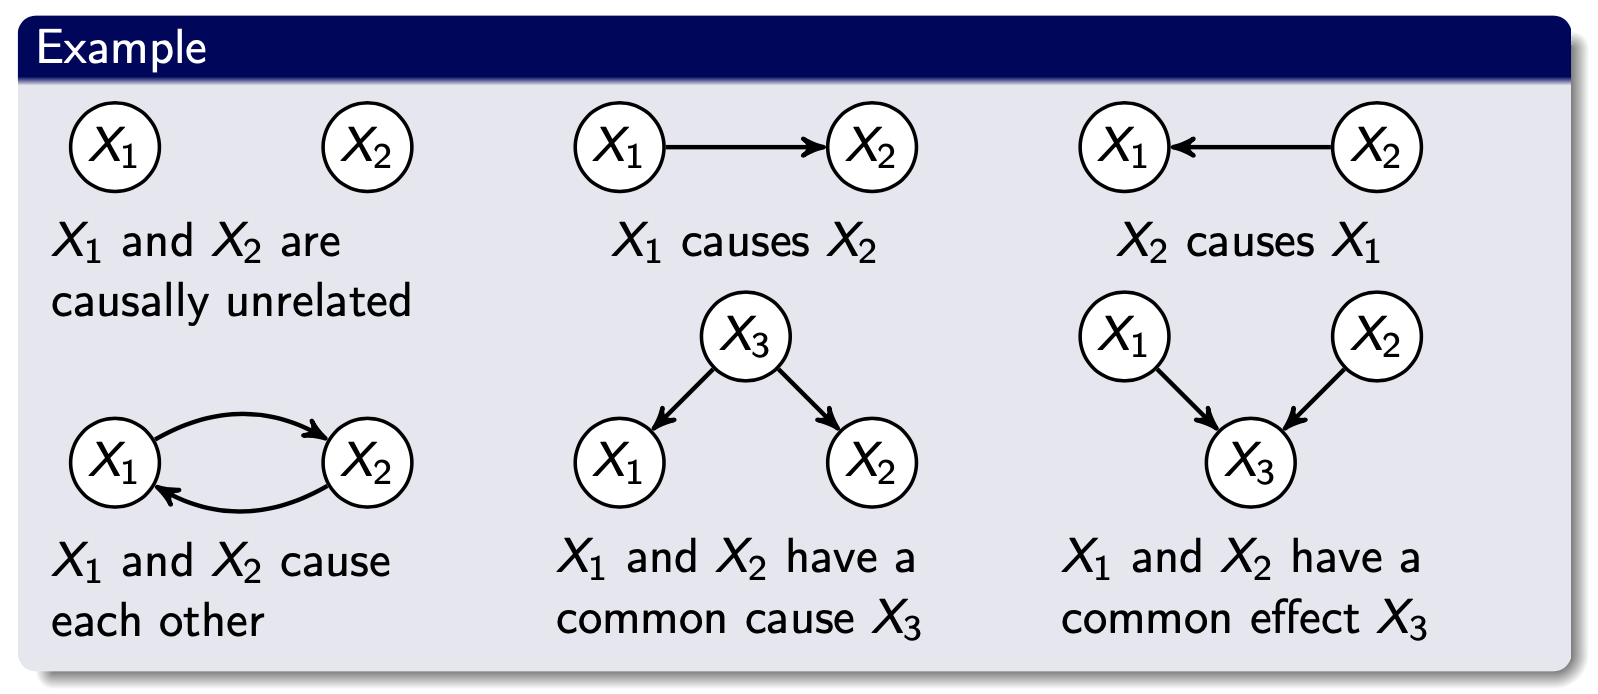
\includegraphics[width=0.6\textwidth]{figures/causality_overview_causal_graphs.png}
		\caption{Examples of causal graphs (retrieved from lecture notes).}
		\label{fig:causality_overview_causal_graphs}
	\end{figure}
	
	Note that these graphs can contain loops, which represents a feedback loop (a change in $A$ leads to a change in $B$, and a change in $B$ leads to a change in $A$). However, we will not take a closer look at those.
	
	\item We can interpreted node relationships in the graph as causal relations:
	\begin{itemize}
		\item $A$ is a \textit{parent} of $B$ $\implies$ $A$ is a direct cause of $B$
		\item $A$ is a \textit{child} of $B$ $\implies$ $A$ is a direct effect of $B$
		\item $A$ is a \textit{ancestor} of $B$ (e.g. $A\to C \to B$) $\implies$ $A$ is a cause of $B$. Note that if we fix $C$, there is no effect of $A$ on $B$. Hence, there is no direct edge.
		\item $A$ is a \textit{descendant} of $B$ (e.g. $B\to C\to A$) $\implies$ $A$ is an effect of $B$.
	\end{itemize}
	\item We use the notation $\mathcal{G}_{\overline{X}}$ to denote a sub-graph of $\mathcal{G}$ in which the incomming edges of $X$ are removed. This is useful for discussing when $X$ is set externally (hence, no influence of parents of $X$ in that case).
	
	Similarly, $\mathcal{G}_{\underline{X}}$ is $\mathcal{G}$ without the outgoing edges of $X$.
	\item  A \textbf{perfect intervention} $\Cdo(X=\xi)$ means that we force $X$ to eb the value $\xi$. Thereby, the graph $\mathcal{G}$ changes to $\mathcal{G}_{\overline{X}}$
	\begin{itemize}
		\item To perform intervention, we require \textit{modularity}, meaning that we can manipulate $X$ without influencing any other variables in the graph $\bm{V}\setminus X$
		\item This can be a challenge in real systems, but in our theoretical models, we can assume that we are able to do so
	\end{itemize}
	\item A variable $H$ is a \textbf{confounder} of $X$ and $Y$ (i.e. $H$ confounds $X$ and $Y$) if there is a directed path from $H$ to $X$ which does not include $Y$, and same from $H$ to $Y$. Note that it is still allowed to have other paths between $X$ and $Y$. Examples of confounders are shown in Figure~\ref{fig:causality_confounders_examples}.
	
	\begin{figure}[ht!]
		\centering
		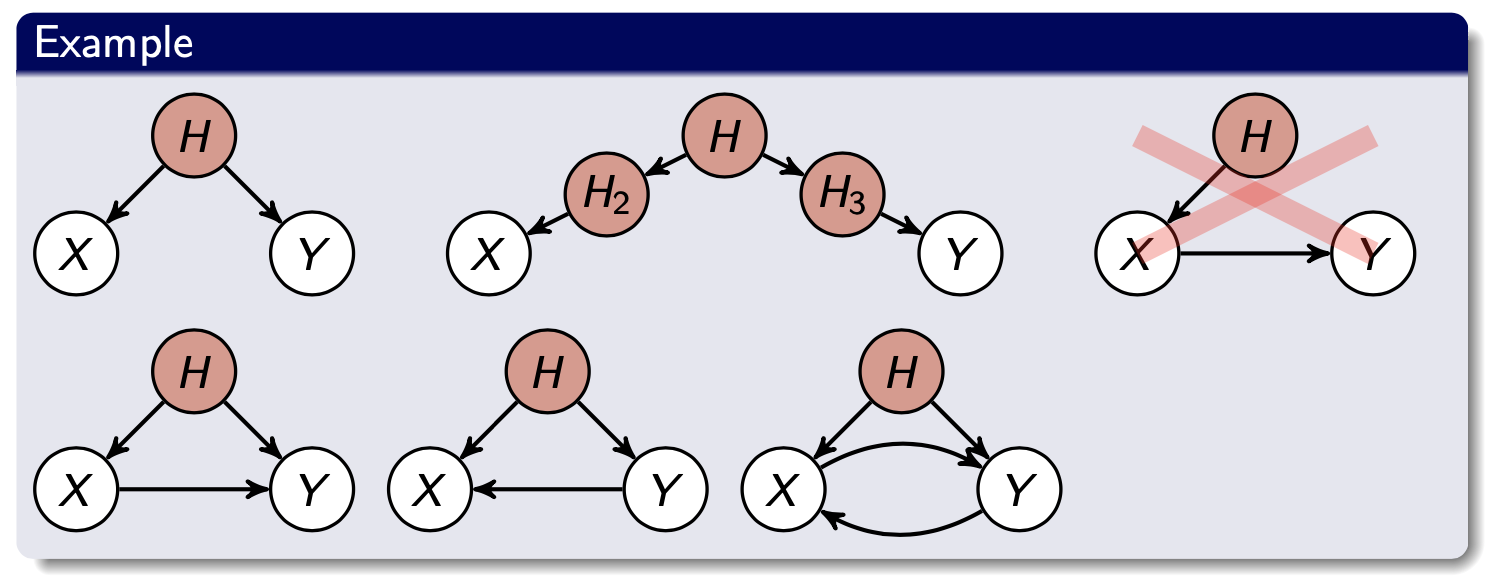
\includegraphics[width=0.5\textwidth]{figures/causality_confounders_examples.png}
		\caption{Examples of when a node $H$ is a confounder of $X$ and $Y$ (retrieved from lecture notes).}
		\label{fig:causality_confounders_examples}
	\end{figure}

	\item \textbf{Reichenbach's principle} sets correlation and causality into relation: if $X$ and $Y$ are correlated/depending on each other, then there is either a causal relation of the type $X\to Y$, $Y\to X$ or there exists a confounder $H$ of $X$ and $Y$.
	\begin{itemize}
		\item Note that this principle can fail is we have a selection bias, meaning that the dataset of $X$ and $Y$ was obtained by only including samples that are conditional on some (possibly latent) event.
	\end{itemize}
\end{itemize}

\subsection{Causal Bayesian Networks}
\begin{itemize}
	\item An subspace of causal networks with many assumptions/limitations, but therefore easier to work with, are Causal Bayesian Networks. We make the following assumptions:
	\begin{itemize}
		\item No confounding % A graph $\mathcal{G}$ does not contain any confounder
		\item A graph $\mathcal{G}$ does not contain any loops
		\item We do not have any selection bias in the data, nor measurements error or time dependencies
	\end{itemize}
	\item We call a Bayesian Network causal if:
	\begin{itemize}
		\item Directed edges correspond with directed causal relations
		\item After a perfect intervention $\Cdo(X_{I}=x_I)$, the probability density becomes:
		\begin{equation*}
		\tcbox[nobeforeafter]{\(
			\begin{split}
				p\left(\bm{X}_{\bm{V}\setminus I}|\Cdo(X_I=x_I)\right) = \prod_{i\in \bm{V}\setminus I} p\left(x_i|\bm{x}_{\text{pa}_i}\right)
			\end{split}
			\)}
		\end{equation*}
		
	\end{itemize}
\end{itemize}

\subsection{Causal Reasoning}
\begin{itemize}
	\item The goal of causal reasoning is to estimate $p(y|\Cdo(X=x))$. If we can express it in terms of the observational distribution $p(x,y,...)$ we say it is \textbf{identifiable} from the observational distribution. 
	
	Note that it does not necessarily require all variables to be observable.
	\item Assume we have the following Bayesian Causal Network:
	
	\begin{figure}[ht!]
		\centering
		\tikz{ %
			\node[latent] (X) {$X$} ; %
			\node[latent, right=of X] (H) {$H$} ; %
			\node[latent, below=of H] (Y) {$Y$} ; %
			
			\edge{H}{X};
			\edge{H}{Y};
			\edge{X}{Y};
		}
	\end{figure}

	The standard conditional distribution is:
	$$p(y|x)=\int p(y|h,x)p(h|x)dh$$

	Now, assume we perform a perfect intervention on $X$, i.e. $\Cdo(X=x)$. What happens is that we neglect the effect of $H$ on $X$, \textit{but} we still need to consider the effect of $H$ on $Y$. Hence, the conditional becomes:
	$$p(y|\Cdo(X=x))=\int p(h)p(y|h,x)dh$$
	The important thing is that we have to prevent that changing $X$ influences $H$ by ``back-reasoning'' (i.e. $H$ causes $X$, but observing $X$ gives us information of $H$), which again influence $Y$. This is because we cannot change $H$ by just forcing $X$ to a value, as we \textit{overwrite} the effect of $H$ on $X$. Hence, we have to explicitly remove its dependency on $X$ in the integral.
	
	%The result indicates that we had to \textit{adjust} the conditional probability for the effect of $H$. But suppose, we would not have the connection between $H$ and $Y$. Then, we would not have to adjust for $H$, and get $p(y|\Cdo(X=x))=p(y|x)$.
	\item We can derive a more general algorithm for deciding, for which variables we need to \textit{adjust} our conditional probability for. This can be done in a very similar manner to d-separation, as we need to find all variables, that are implicitly changed by setting $X$ to a certain value (i.e. variables that influence the decision of which value $X$ can have), but then also influence $Y$. We do not want this influence because by forcing $X$ to be a certain value, we cannot change variables that cause $X$. Hence, we are trying to find a set of variables $S$ which break these kind of influences, and remove their dependency with $X$.
	
	\item In general, we can determine whether $S$ is a sufficient set of variables we are adjusting by the following check:
	
	\begin{tcolorbox}[colback=white!80!gray,colframe=gray!75!black,title=Back-door criterion]
		A set of variables $S$ satisfies the back-door criterion relative to a variable pair ($X$, $Y$), if:
		\begin{enumerate}
			\item $X, Y\not\in S$
			\item No node of $S$ is a descendant (i.e. child of a child etc.) of $X$
			\item $S$ blocks all paths from $Y$ to $X$ where we have an incoming edge to $X$ (other directions irrelevant for path itself). A path is blocked by $S$ if:
			\begin{enumerate}
				\item It contains a collider $...\rightarrow u \leftarrow ...$ such that $u$ is not an ancestor of a node in $S$
				\item It contains a non-collider $...\rightarrow u$, $...\rightarrow u \rightarrow ...$, $...\leftarrow u \rightarrow ...$ such that $u$ is in $S$
			\end{enumerate}
		\end{enumerate}
		Then $S$ is admissible for adjustment to find the causal effect of $X$ on $Y$:
		$$p(y|\Cdo(X=x))=\int p(y|X=x,S=s)p(S=s)ds$$
		If $S=\emptyset$: $p(y|\Cdo(X=x))=p(y|X=x)$
	\end{tcolorbox}	

	To find the actual set $S$, we can simply perform the algorithm backwards. First, find all paths from $Y$ to $X$ with an incoming edge to $X$. Then, we start with $S=\emptyset$, and try to block all paths by adding variables to $S$. In case that all paths were blocked from the beginning on, or no paths exist, we can stop with $S=\emptyset$.
	
	\item \underline{Examples}: 
	\begin{itemize}
		\item Consider the examples in Figure~\ref{fig:causality_backdoor_example}. Note that we usually try to find the smallest set of admissible variables as this simplifies the integral we have to take.
		
		\begin{figure}[ht!]
			\centering
			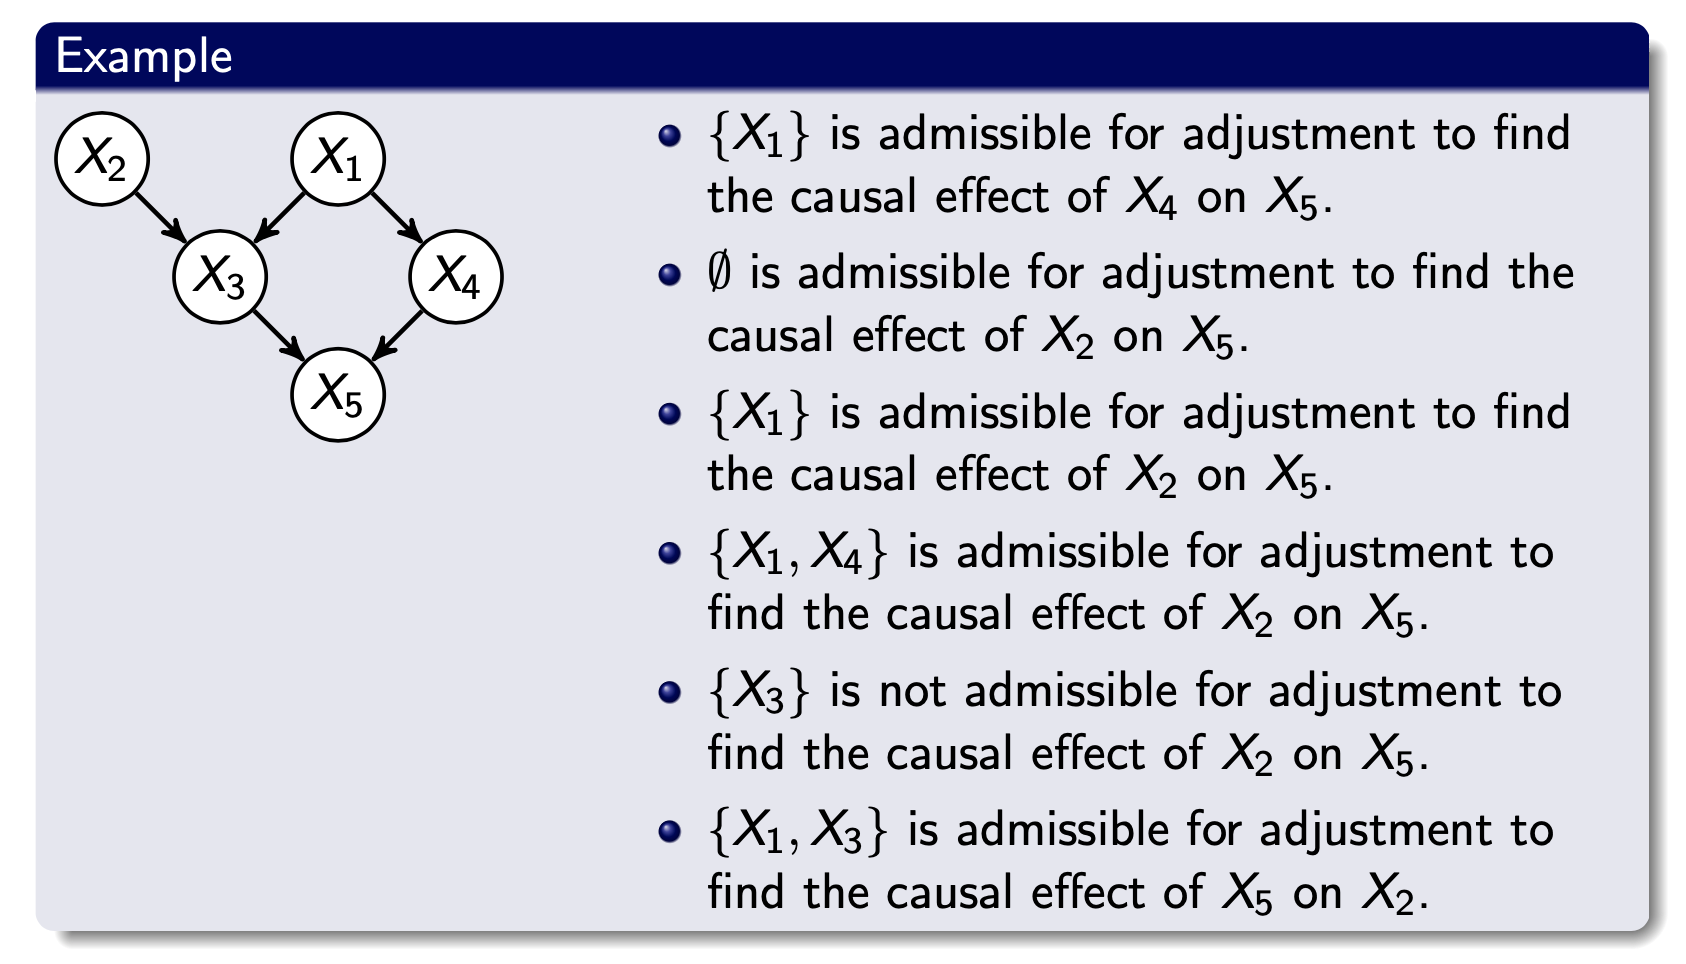
\includegraphics[width=0.5\textwidth]{figures/causality_backdoor_example.png}
			\caption{Example of admissible sets of variables for adjustment (retrieved from lecture notes).}
			\label{fig:causality_backdoor_example}
		\end{figure}
		\newpage
		\item Consider the following, slightly more complicated Causal Bayesian Network:
		\begin{figure}[ht!]
			\centering
			\tikz{ %
				\node[latent] (X1) {$X_1$} ; %
				\node[latent, below=of X1] (X3) {$X_3$} ; %
				\node[latent, right=of X3] (X4) {$X_4$} ; %
				\node[latent, right=of X4] (X5) {$X_5$} ; %
				\node[latent, above=of X5] (X2) {$X_2$} ; %
				\node[latent, below=of X3] (X7) {$X_7$} ; %
				\node[latent, right=of X7] (X6) {$X_6$} ; %
				\node[latent, right=of X6] (X8) {$X_8$} ; %
				
				\edge{X1}{X3};
				\edge{X1}{X4};
				\edge{X3}{X7};
				\edge{X4}{X7};
				\edge{X4}{X8};
				\edge{X7}{X6};
				\edge{X6}{X8};
				\edge{X5}{X8};
				\edge{X2}{X5};
				\edge{X2}{X4};
			}
		\end{figure}	
	
		We are trying to find the set $S$ admissible for adjustment for the causal effect of $X_7$ on $X_8$ (the two nodes on the bottom, left and right). We have to consider all paths with incoming edges to $X_7$, so from $X_3$ and $X_4$. To block the path $X_8\to X_4\to X_7$, we add $X_4$ to $S$: $S=\{X_4\}$. However, by doing this, we unblocked another path: $X_8\to X_5\to X_2\to X_4\to X_1\to X_3\to X_7$. $X_4$ is not longer a collider anymore, as it is included in $S$. So, we can either add $X_3$, or $X_5$, or even $X_1$ or $X_2$ to block this path. For example, we can take $S=\{X_3,X_4\}$, which is then admissible for adjustment as all paths are blocked.
	\end{itemize}
	\item Although we found a way to estimate what happens when we perform an intervention, the best way to find causal relations is to use randomized controlled trials. In a drug test, this would mean that we completely random assign a person to take the drug or not, ensuring that no underlying selection bias is in the process. By that, we should break all back-door paths (as there is nothing besides a coin flip that causes the event of  "taking the drug")

\end{itemize}
\appendix
\newpage
\section{Appendix Math}
Here we revisit some important mathematical tricks and equations to know.  
\subsection{Useful properties of a Gaussian}
Given $\bm{x}\sim \mathcal{N}(\bm{\mu}, \bm{\Sigma})$, suppose $\bm{x}=(\bm{x}_a, \bm{x}_b)$, define $\bm{\mu}=(\bm{\mu}_a, \bm{\mu}_b)$ and $\bm{\Sigma} = \begin{bmatrix}
\Sigma_{aa} & \Sigma_{ab}\\ \Sigma_{ba} & \Sigma_{bb}
\end{bmatrix}$ ($\Sigma_{ab}=\Sigma_{ba}^T$, $\Sigma_{aa}=\Sigma_{aa}^T$)\\

\textbf{Marginal distribution}: $p(\bm{x}_a) = \mathcal{N}(\bm{x}_a\mid \bm{\mu}_a, \Sigma_{aa})$\\

\textbf{Conditional distribution}: $p(\bm{x}_a\vert \bm{x}_b) = \mathcal{N}(\bm{x}_a\mid \bm{\mu}_{a|b}, \Sigma_{a|b})$\\ where $\Sigma_{a|b} = \Sigma_{aa} - \Sigma_{ab}\Sigma_{bb}^{-1}\Sigma_{ba}, \bm{\mu}_{a\vert b} = \bm{\mu}_a + \Sigma_{ab}\Sigma_{bb}^{-1}\left(\bm{x}_{b}-\bm{\mu}_{b}\right)$\\[10pt]

\textbf{Multiplication of two Gaussians}: $\mathcal{N}(\bm{x}\mid \bm{a}, \bm{A})\mathcal{N}(\bm{x}\mid\bm{b}, \bm{B})=\mathcal{N}(\bm{x}|\bm{c}, \bm{C})\overbrace{\mathcal{N}(\bm{a}|\bm{b}, \bm{A}+\bm{B})}^{\text{Normalization constant}}$\\ where $\bm{C}=\left(\bm{A}^{-1}+\bm{B}^{-1}\right)^{-1}$, $\bm{c}=\bm{C}\left(\bm{A}^{-1}\bm{a}+\bm{B}^{-1}\bm{b}\right)$\\

\textbf{Conditional and marginals in graphical model}\\
\begin{wrapfigure}[3]{l}{0.1\textwidth}
	\centering
	\tikz{ %
		\node[latent] (x) {$\bm{x}$} ; %
		\node[latent, below=of x] (y) {$\bm{y}$} ; %
		
		\edge{x}{y}
	}
\end{wrapfigure}
\begin{equation*}
	\begin{split}
		p(x) & = \mathcal{N}(x|\mu, \Lambda^{-1})\\
		p(y|x) & = \mathcal{N}(Ax+b, L^{-1})\\[10pt]
		\Rightarrow p(y) & = \mathcal{N}(y|A\mu + b, L^{-1} + A\Lambda^{-1}A^T)\\
		\Rightarrow p(x|y) & = \mathcal{N}(x|\Sigma(A^T L (y - b) + \Lambda\mu), \Sigma), \hspace{2mm} \Sigma=(\Lambda + A^T L A)^{-1}
	\end{split}
\end{equation*}


\subsection{Distributions from the exponential family}
It is useful to know the exponential form of a few most popular distributions. Remember that in general, a distribution of the exponential family can be written in the form:
$$p(\bm{x}|\bm{\eta}) = h(\bm{x})g(\bm{\eta})\exp\left(\bm{\eta}^T \cdot \bm{u}(\bm{x})\right)$$
Some tricks to keep in mind:
\begin{itemize}
	\item $a^{b}=\exp(b\cdot \log a)$ - helpful to find sufficient statistics and natural parameters
	\item If we have the constraint $\sum_k \pi_k= 1$, replace $\pi_K$ with $\pi_K=1-\sum_{k\neq K} \pi_k$ $\Rightarrow$ one less parameter
\end{itemize}
\subsubsection{Gaussian}
\textbf{Univariate}:
\begin{fleqn}[\parindent]
	\begin{equation*}
	\begin{split}
	& p(x|\mu, \sigma^2) = \mathcal{N}(x|\mu, \sigma^2) = \frac{1}{\sqrt{2\pi}\sigma}\exp\left(-\frac{(x-\mu)^2}{2\sigma^2}\right)\\[8pt]
	& \bm{\eta} = \begin{bmatrix}
	\frac{\mu}{\sigma^2} & -\frac{1}{2\sigma^2}\\
	\end{bmatrix}^T\\
	& \bm{u}(\bm{x}) = \begin{bmatrix}
	x & x^2\\
	\end{bmatrix}^T\\
	& h(\bm{x}) = \frac{1}{\sqrt{2\pi}}\\
	& g(\bm{\eta}) = \frac{1}{\sigma}\exp\left(-\frac{\eta_1^2}{4\cdot \eta_2}\right)\\
	\end{split}
	\end{equation*}
\end{fleqn}
\textbf{Multivariate}:
\begin{fleqn}[\parindent]
	\begin{equation*}
		\begin{split}
			& p(\bm{x}|\bm{\mu}, \bm{\Sigma}) = \mathcal{N}(\bm{x}|\bm{\mu}, \bm{\Sigma}) = (2\pi)^{-D/2}|\Sigma|^{-1}\cdot \exp\left(-\frac{1}{2}(\bm{x}-\bm{\mu})^T\Sigma^{-1}(\bm{x}-\bm{\mu})\right)\\[8pt]
			& \bm{\eta} = \begin{bmatrix}
			\bm{\Sigma}^{-1}\bm{\mu} & -\frac{1}{2}\bm{\Sigma}^{-1}\\
			\end{bmatrix}^T\\
			& \bm{u}(\bm{x}) = \begin{bmatrix}
				\bm{x} & \bm{x}\bm{x}^T\\
			\end{bmatrix}^T\\
			& h(\bm{x}) = (2\pi)^{-D/2}\\
			& g(\bm{\eta}) = |-2\bm{\eta}_1| \cdot \exp\left(\frac{1}{4}\bm{\eta}_{1}^T\bm{\eta}_{2}^{-1}\bm{\eta}_{1}\right)\\
		\end{split}
	\end{equation*}
\end{fleqn}
\subsubsection{Beta}
\begin{fleqn}[\parindent]
	\begin{equation*}
	\begin{split}
	& p(x|\alpha, \beta) = \frac{x^{\alpha-1}(1 - x)^{\beta-1}}{B(\alpha, \beta)} \hspace{4mm}\text{where}\hspace{4mm}B(\alpha, \beta)=\frac{\Gamma(\alpha)\Gamma(\beta)}{\Gamma(\alpha + \beta)}\\[8pt]
	& \bm{\eta} = \begin{bmatrix}
	\alpha & \beta\\
	\end{bmatrix}^T\\
	& \bm{u}(\bm{x}) = \begin{bmatrix}
	\log x & \frac{1}{x}\\
	\end{bmatrix}^T\\
	& h(\bm{x}) = 1\\
	& g(\bm{\eta}) = \frac{1}{B(\eta_1, \eta_2)}\\
	\end{split}
	\end{equation*}
\end{fleqn}
\subsubsection{Multinomial}
\begin{fleqn}[\parindent]
	\begin{equation*}
	\begin{split}
	& p(\bm{x}|\bm{\pi}) = \frac{M!}{\prod_{i=1}^{K}x_i!}\prod_{i=1}^{K}\pi_i^{x_i}\\[8pt]
	& \bm{\eta} = \begin{bmatrix}
	\ln\frac{\pi_1}{1-\sum_{i=1}^{K-1}\pi_i} & \ln\frac{\pi_2}{1-\sum_{i=1}^{K-1}\pi_i} & ... & \ln\frac{\pi_{K-1}}{1-\sum_{i=1}^{K-1}\pi_i}
	\end{bmatrix}^T\\
	& \bm{u}(\bm{x}) = \begin{bmatrix}
	x_1 & x_2 & ... & x_{K-1}
	\end{bmatrix}^T\\
	& h(\bm{x}) = \frac{M!}{\prod_{i=1}^{K}x_i!}\\
	& g(\bm{\eta}) = \exp\left(-M\ln \left(1 + \sum_{i=1}^{K-1}\exp(\eta_i)\right)\right)\\
	\end{split}
	\end{equation*}
\end{fleqn}
\subsubsection{Dirichlet}
\begin{fleqn}[\parindent]
	\begin{equation*}
	\begin{split}
	& p(\bm{x}|\alpha_1,..,\alpha_K) = \frac{1}{B(\alpha_1,..., \alpha_K)}\prod_{i=1}^{K}x_i^{\alpha_i-1} \hspace{4mm}\text{where}\hspace{4mm}B(\alpha_1,...,\alpha_K)=\frac{\prod_{i=1}^{K}\Gamma(\alpha_i)}{\Gamma(\sum_{i=1}^{K} \alpha_i)}\\[8pt]
	& \bm{\eta} = \begin{bmatrix}
	\alpha_1 & ... & \alpha_K\\
	\end{bmatrix}^T\\
	& \bm{u}(\bm{x}) = \begin{bmatrix}
	\log x_1 & ... & \log x_K\\
	\end{bmatrix}^T\\
	& h(\bm{x}) = \frac{1}{\prod_{i=1}^{K}x_i}\\
	& g(\bm{\eta}) = \frac{1}{B(\eta_1, ..., \eta_K)}\\
	\end{split}
	\end{equation*}
\end{fleqn}
\subsubsection{Poisson}
\begin{fleqn}[\parindent]
	\begin{equation*}
	\begin{split}
	& p(x|\lambda) = \frac{\lambda^{x}\exp(-x)}{x!}\\[8pt]
	& \bm{\eta} = \begin{bmatrix}
	\ln \lambda \\
	\end{bmatrix}^T\\
	& \bm{u}(\bm{x}) = \begin{bmatrix}
	x\\
	\end{bmatrix}^T\\
	& h(\bm{x}) = \frac{1}{x!}\\
	& g(\bm{\eta}) = \exp(-\exp(\eta))\\
	\end{split}
	\end{equation*}
\end{fleqn}
\subsubsection{Gamma}
\begin{fleqn}[\parindent]
	\begin{equation*}
	\begin{split}
	& p(x|a,b) = \frac{1}{\Gamma(x)}b^{a}x^{a-1}\exp(-bx)\\[8pt]
	& \bm{\eta} = \begin{bmatrix}
	(a-1) & -b \\
	\end{bmatrix}^T\\
	& \bm{u}(\bm{x}) = \begin{bmatrix}
	\ln x & x\\
	\end{bmatrix}^T\\
	& h(\bm{x}) = 1\\
	& g(\bm{\eta}) = \frac{(-\eta_2)^{\eta_1+1}}{\Gamma(\eta_1+1)}\\
	\end{split}
	\end{equation*}
\end{fleqn}
\subsubsection{Conjugate priors}
\begin{itemize}
	\item Dirichlet $\to$ Multinomial 
	\item Dirichlet $\to$ Categorical 
	\item Beta $\to$ Bernoulli
	\item Gamma $\to$ Poisson
	\item Gaussian $\to$ Gaussian
	\item Gamma (precision) $\to$ Gaussian (known mean)
\end{itemize}

\end{document}